\documentclass[10pt, aspectratio=43]{beamer}

% --- Pacotes Básicos ---
\usepackage[utf8]{inputenc}
\usepackage[T1]{fontenc}
\usepackage[brazilian]{babel}
\usepackage{amsmath, amssymb, amsthm}
\usepackage{listings}
\usepackage{xcolor}
\usepackage{tikz}
\usepackage{tcolorbox}
\usepackage{booktabs} % \toprule, \midrule, \bottomrule usados na tabela de resultados
\usepackage{array}
\newcolumntype{L}[1]{>{\raggedright\arraybackslash}p{#1}}
\usepackage[alf]{abntex2cite}
\setbeamertemplate{caption}[numbered]

% --- Configuração Visual IDÊNTICA ao PDF 09-logic-in-lean ---
\usetheme{Singapore} % Tema nativo que gera o degradê e os miniframes exatamente como no PDF
\setbeamertemplate{navigation symbols}{} % Remove ícones de navegação inferiores

% Cores originais do Beamer/PDF
\definecolor{pucblue}{RGB}{51, 51, 179} % Azul clássico do Beamer (structure) usado no PDF
\definecolor{commentgreen}{RGB}{0, 110, 0}
\definecolor{keywordblue}{RGB}{0, 0, 180}

\setbeamercolor{structure}{fg=pucblue}
\setbeamercolor{title}{fg=pucblue}
\setbeamercolor{frametitle}{fg=pucblue}
\setbeamercolor{section in head/foot}{fg=pucblue}

% Ajusta a cor do degradê do tema Singapore para o tom suave do PDF
\colorlet{beamer@blendedblue}{pucblue}

% Estilo reutilizável para as caixas (tcolorbox); evita repetir as cores em cada slide
\tcbset{
  pucbox/.style={colback=pucblue!5!white, colframe=blue!75!black}
}

% --- Bolinhas vazadas no cabeçalho e marcadores redondos ---
\setbeamertemplate{mini frames}[circle]
\setbeamertemplate{itemize items}[circle]
\setbeamertemplate{enumerate items}[default]
\setbeamertemplate{sections/subsections in toc}[sections numbered]

% Título dos slides alinhado à esquerda (o tema Singapore centraliza por padrão)
\setbeamertemplate{frametitle}[default][left]

% Rodapé limpo apenas com numeração X/Y em negrito na direita (oculto quando sem número)
\setbeamertemplate{footline}{%
  \hfill \textbf{\insertframenumber/\inserttotalframenumber} \hspace{0.3cm} \vspace{0.2cm}
}

% Slide de Sumário automático no início de cada seção (sem contar nem exibir número de página, igual ao PDF)
\AtBeginSection[]{
  {
    \setbeamertemplate{footline}{}
    \begin{frame}[noframenumbering]{Sumário}
      \tableofcontents[currentsection]
    \end{frame}
  }
}

% --- Configuração de Caixas de Código para Lean 4 (Fundo branco e borda fina, igual ao PDF) ---
\lstdefinelanguage{Lean4}{
  keywords={def, abbrev, theorem, lemma, example, structure, inductive, where, by, match, intro, apply, exact, rw, cases, with, assumption, rfl, sorry, exfalso, contradiction, forall, exists, Prop, Type, Nat, Bool, List, False, True, And, Or, Not, Injective},
  keywordstyle=\color{keywordblue}\bfseries,
  comment=[l]{--},
  commentstyle=\color{commentgreen}\ttfamily,
  basicstyle=\ttfamily\footnotesize\color{pucblue!90!black},
  backgroundcolor=\color{white},
  frame=single,
  rulecolor=\color{black},
  framesep=4pt,
  xleftmargin=4pt,
  xrightmargin=4pt,
  showstringspaces=false,
  breaklines=true,
  literate=
    {→}{{$\rightarrow$}}1
    {←}{{$\leftarrow$}}1
    {↔}{{$\leftrightarrow$}}1
    {∀}{{$\forall$}}1
    {∃}{{$\exists$}}1
    {∧}{{$\wedge$}}1
    {∨}{{$\vee$}}1
    {¬}{{$\neg$}}1
    {≠}{{$\neq$}}1
    {≤}{{$\le$}}1
    {≥}{{$\ge$}}1
    {α}{{$\alpha$}}1
    {β}{{$\beta$}}1
    {ℕ}{{$\mathbb{N}$}}1
    {∞}{{$\infty$}}1
    {∣}{{$\mid$}}1
    {ç}{{\c{c}}}1
    {ã}{{\~a}}1
}

% --- Metadados da Apresentação (Formatação nativa idêntica à capa do PDF) ---
\title[Weak PNT via Kolmogorov em Lean 4]{Formalizando o Teorema Fraco dos Números Primos e seus Refinamentos Iterados via Complexidade de Kolmogorov}
\subtitle{\small{Uma Prova Formalizada pelo Método da Incompressibilidade em Lean 4}}
\author{Gabriel Resende Machado\texorpdfstring{\\[0.2ex]}{, }{\footnotesize INF2290: Tópicos em Teoria da Computação IV -- Formalização em Lean}}
\institute{\small Departamento de Informática, PUC-Rio}
\date{\tikz[remember picture,overlay] \node[anchor=south, yshift=0.5cm] at (current page.south) {10 de Dezembro de 2026};}

\begin{document}

% --- SLIDE DE TÍTULO ---
% Exibe o cabeçalho com degradê, mas omite o número de página no rodapé (como na pág. 1 do PDF)
{
  \setbeamertemplate{footline}{}
  \begin{frame}
    \titlepage
  \end{frame}
}

% --- SUMÁRIO GERAL INICIAL (Igual à pág. 2 do PDF) ---
{
  \setbeamertemplate{footline}{}
  \begin{frame}[noframenumbering]{Sumário}
    \tableofcontents
  \end{frame}
}

% =========================================================================
\section{Introdução}
% =========================================================================

\begin{frame}{O Desafio dos Limites Inferiores}
  Na Teoria da Computação, há uma assimetria fundamental entre dois tipos de problemas:
  \vspace{0.3cm}
  \begin{itemize}
    \item \textbf{Limites Superiores:} para estabelecer um limite superior, basta demonstrar um algoritmo, um circuito ou uma codificação que resolva o problema em espaço ou tempo $T \in O(f(n))$;

    \vspace{2mm}
    \begin{itemize}
        \item O algoritmo \textit{MergeSort} ordena \textit{n} itens com $O(n \log n)$ comparações (afirmação existencial $\exists$).
    \end{itemize}
    
    \vspace{0.2cm}
    \item \textbf{A Dificuldade Assintótica dos Limites Inferiores:} estabelecer um limite inferior $T \in \Omega(f(n))$ exige uma prova universal negativa, \textit{i.e.} demonstrar que \textbf{nenhum} algoritmo possível, sob um determinado modelo computacional, pode ser mais rápido ou compacto que um dado limiar.

    \vspace{2mm}
    \begin{itemize}
        \item Exibir um caminho de 10 km prova que a distância é no máximo 10 km; provar que ela é no mínimo 10 km exige descartar todos os caminhos possíveis (afirmação universal $\forall$).
    \end{itemize}
  \end{itemize}
\end{frame}

\begin{frame}{O Desafio dos Limites Inferiores}
    \begin{figure}
        \centering
        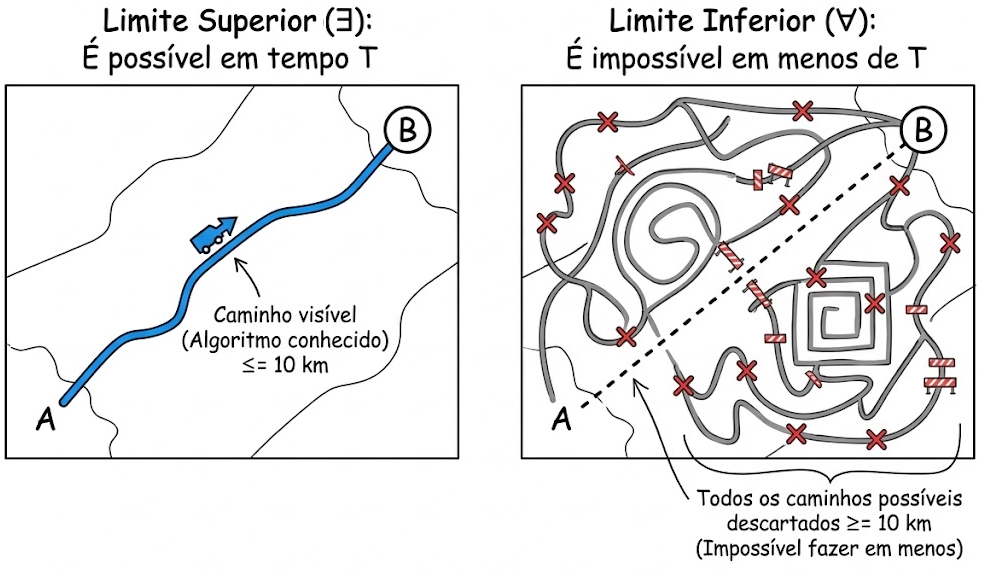
\includegraphics[width=0.95\textwidth]{figures/bounds_example.png}
        \caption{\scriptsize{A assimetria na Teoria da Complexidade. À esquerda, um limite superior prova-se encontrando um único caminho válido. À direita, um limite inferior exige demonstrar que nenhum caminho no universo de possibilidades consegue quebrar a barreira estabelecida.}}
        \label{fig:bounds_example}
    \end{figure}
\end{frame}

\begin{frame}{Regularidade vs. Aleatoriedade}
    \vspace{1mm}
    \begin{itemize}
        \item \small{Um objeto é aleatório se não for possível gerar sua sequência por meio de um programa menor do que ela mesma;}
        \vspace{1mm}
        \item \textbf{\small{Objetos aleatórios são comumente chamados de imcompressíveis via Complexidade de Kolmogorov.}}
    \end{itemize}
    \vspace{1mm}
    \begin{figure}
        \centering
        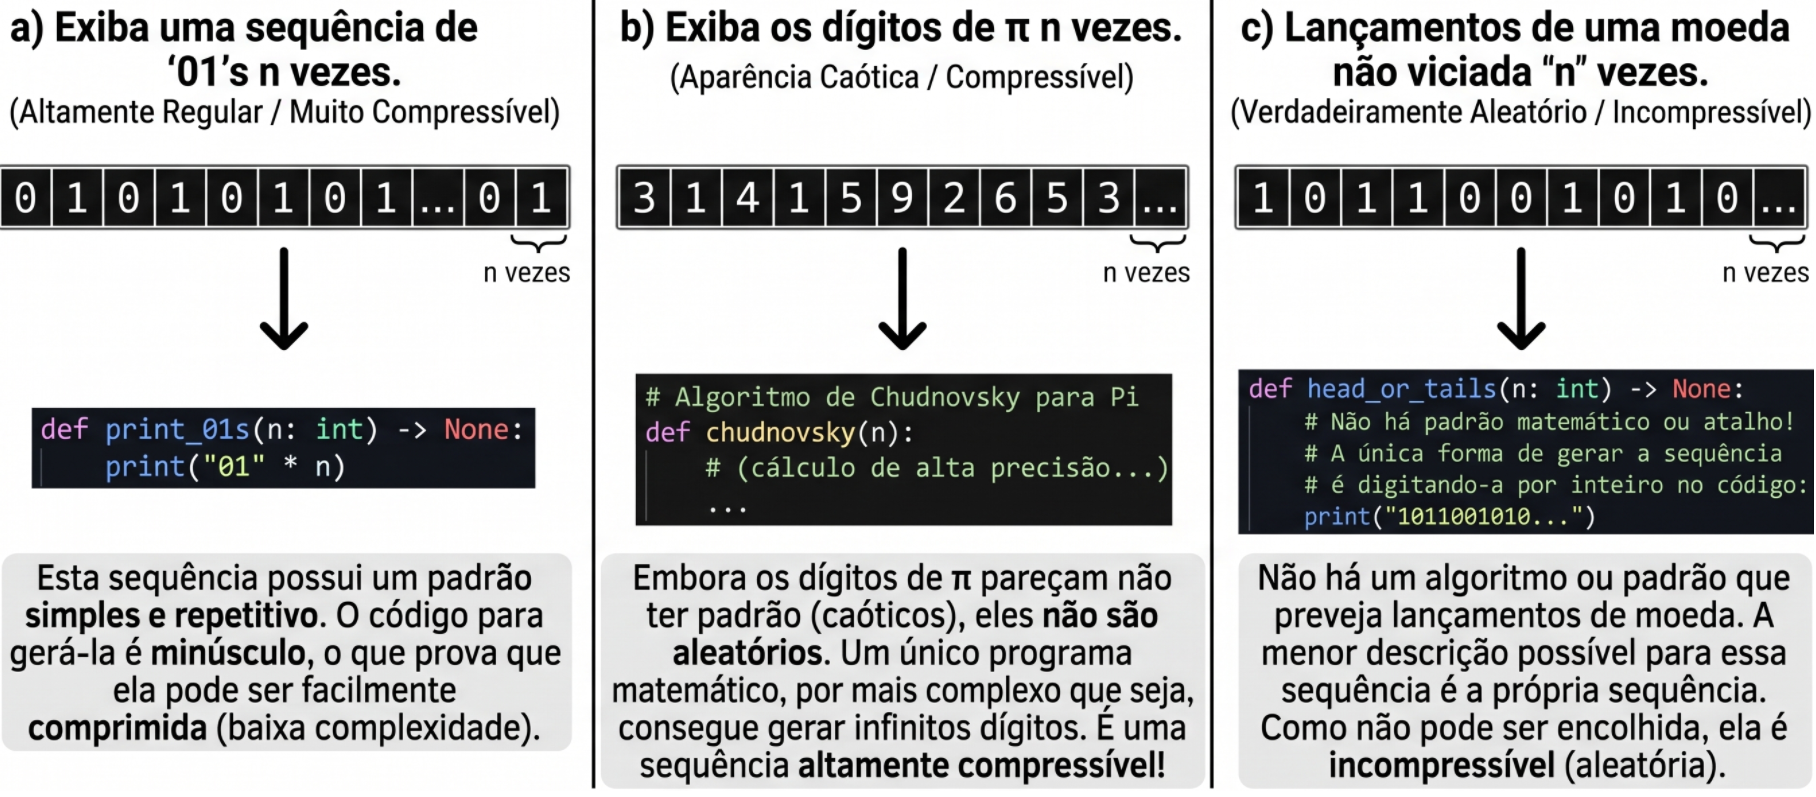
\includegraphics[width=0.98\textwidth]{figures/kolmogorov_examples.png}
        \caption{\footnotesize{Regularidade vs. Aleatoriedade na Complexidade de Kolmogorov: a incompressibilidade algorítmica como a verdadeira medida do que é aleatório.}}
        \label{fig:kolmogorov_examples}
    \end{figure}
\end{frame}

\begin{frame}{A Complexidade de Kolmogorov}
\vspace{2mm}

A Complexidade de Kolmogorov $K(x)$ é o tamanho (em bits) do menor programa que gera $x$, tal que $|x| = n$.

 \begin{tcolorbox}[pucbox, title=Definição Formal]
    \footnotesize{Na Figura \ref{fig:kolmogorov_examples}, nos casos $a)$ e $b)$, as strings de $n$ bits obedeciam a algum padrão ou comportamento reproduzível por meio de um algoritmo de custo adicional $c$ produzir uma saída menor do que $n$. Daí, tem-se:}
    \begin{equation}
        K(x) < n + c
    \end{equation}
    \footnotesize{Contudo, no caso $c)$, não há como reproduzir a saída de $n$ lançamentos de moeda pela sua intrínseca natureza não determinística, a não ser por um algoritmo específico que exiba a própria saída $n$ de lançamentos. Portanto:}
    \begin{equation}
        K(x) \ge n - c
    \end{equation}
    \footnotesize{Como aqui o objetivo é caracterizar sequências que não podem ser significativamente comprimidas, $c$ representa a quantidade máxima de bits que admite-se perder em relação ao comprimento original da sequência.}
 \end{tcolorbox}    
\end{frame}

\begin{frame}{Cenários de Aplicação do Método da Incompressibilidade}
    \small
    \begin{itemize}
        \item O método da incompressibilidade fornece limites inferiores em diversos domínios da Teoria da Computação, como complexidade de circuitos e complexidade temporal de Máquinas de Turing \cite{li2019introduction};
        \item Este trabalho foca no \textbf{Cenário 1}: Teoria dos Números e a Distribuição dos Primos.
    \end{itemize}
    \begin{figure}
        \centering
        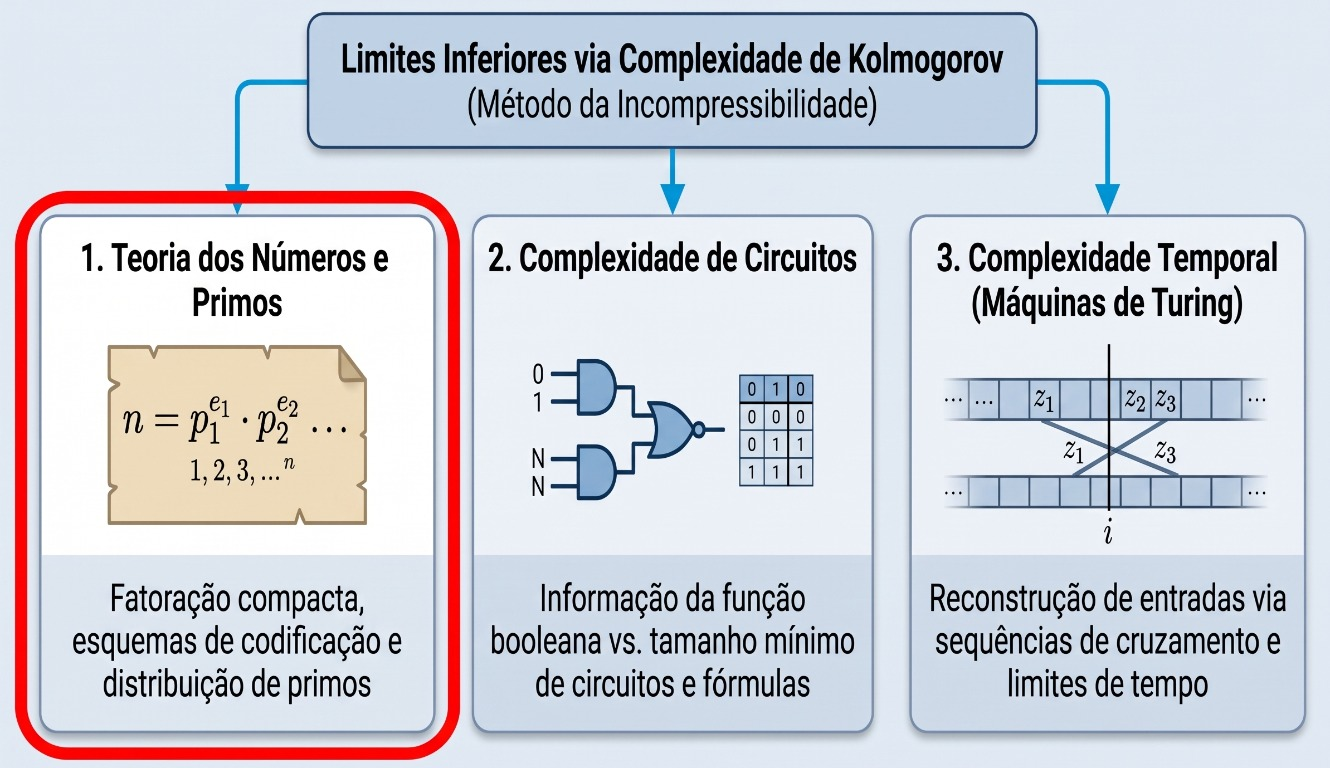
\includegraphics[height=0.47\textheight]{figures/application_scenarios.jpeg}
        \caption{\footnotesize{Cenários de aplicação de limites inferiores via Complexidade de Kolmogorov. Em destaque, o cenário abordado neste trabalho.}}
        \label{fig:application_scenarios}
    \end{figure}
\end{frame}

\begin{frame}{O Princípio da Casa dos Pombos}
\vspace{1mm}
Objetos imcompressíveis -- ou Kolmogorov-Aleatórios -- violam o Princípio da Casa dos Pombos.
    \begin{figure}
        \centering
        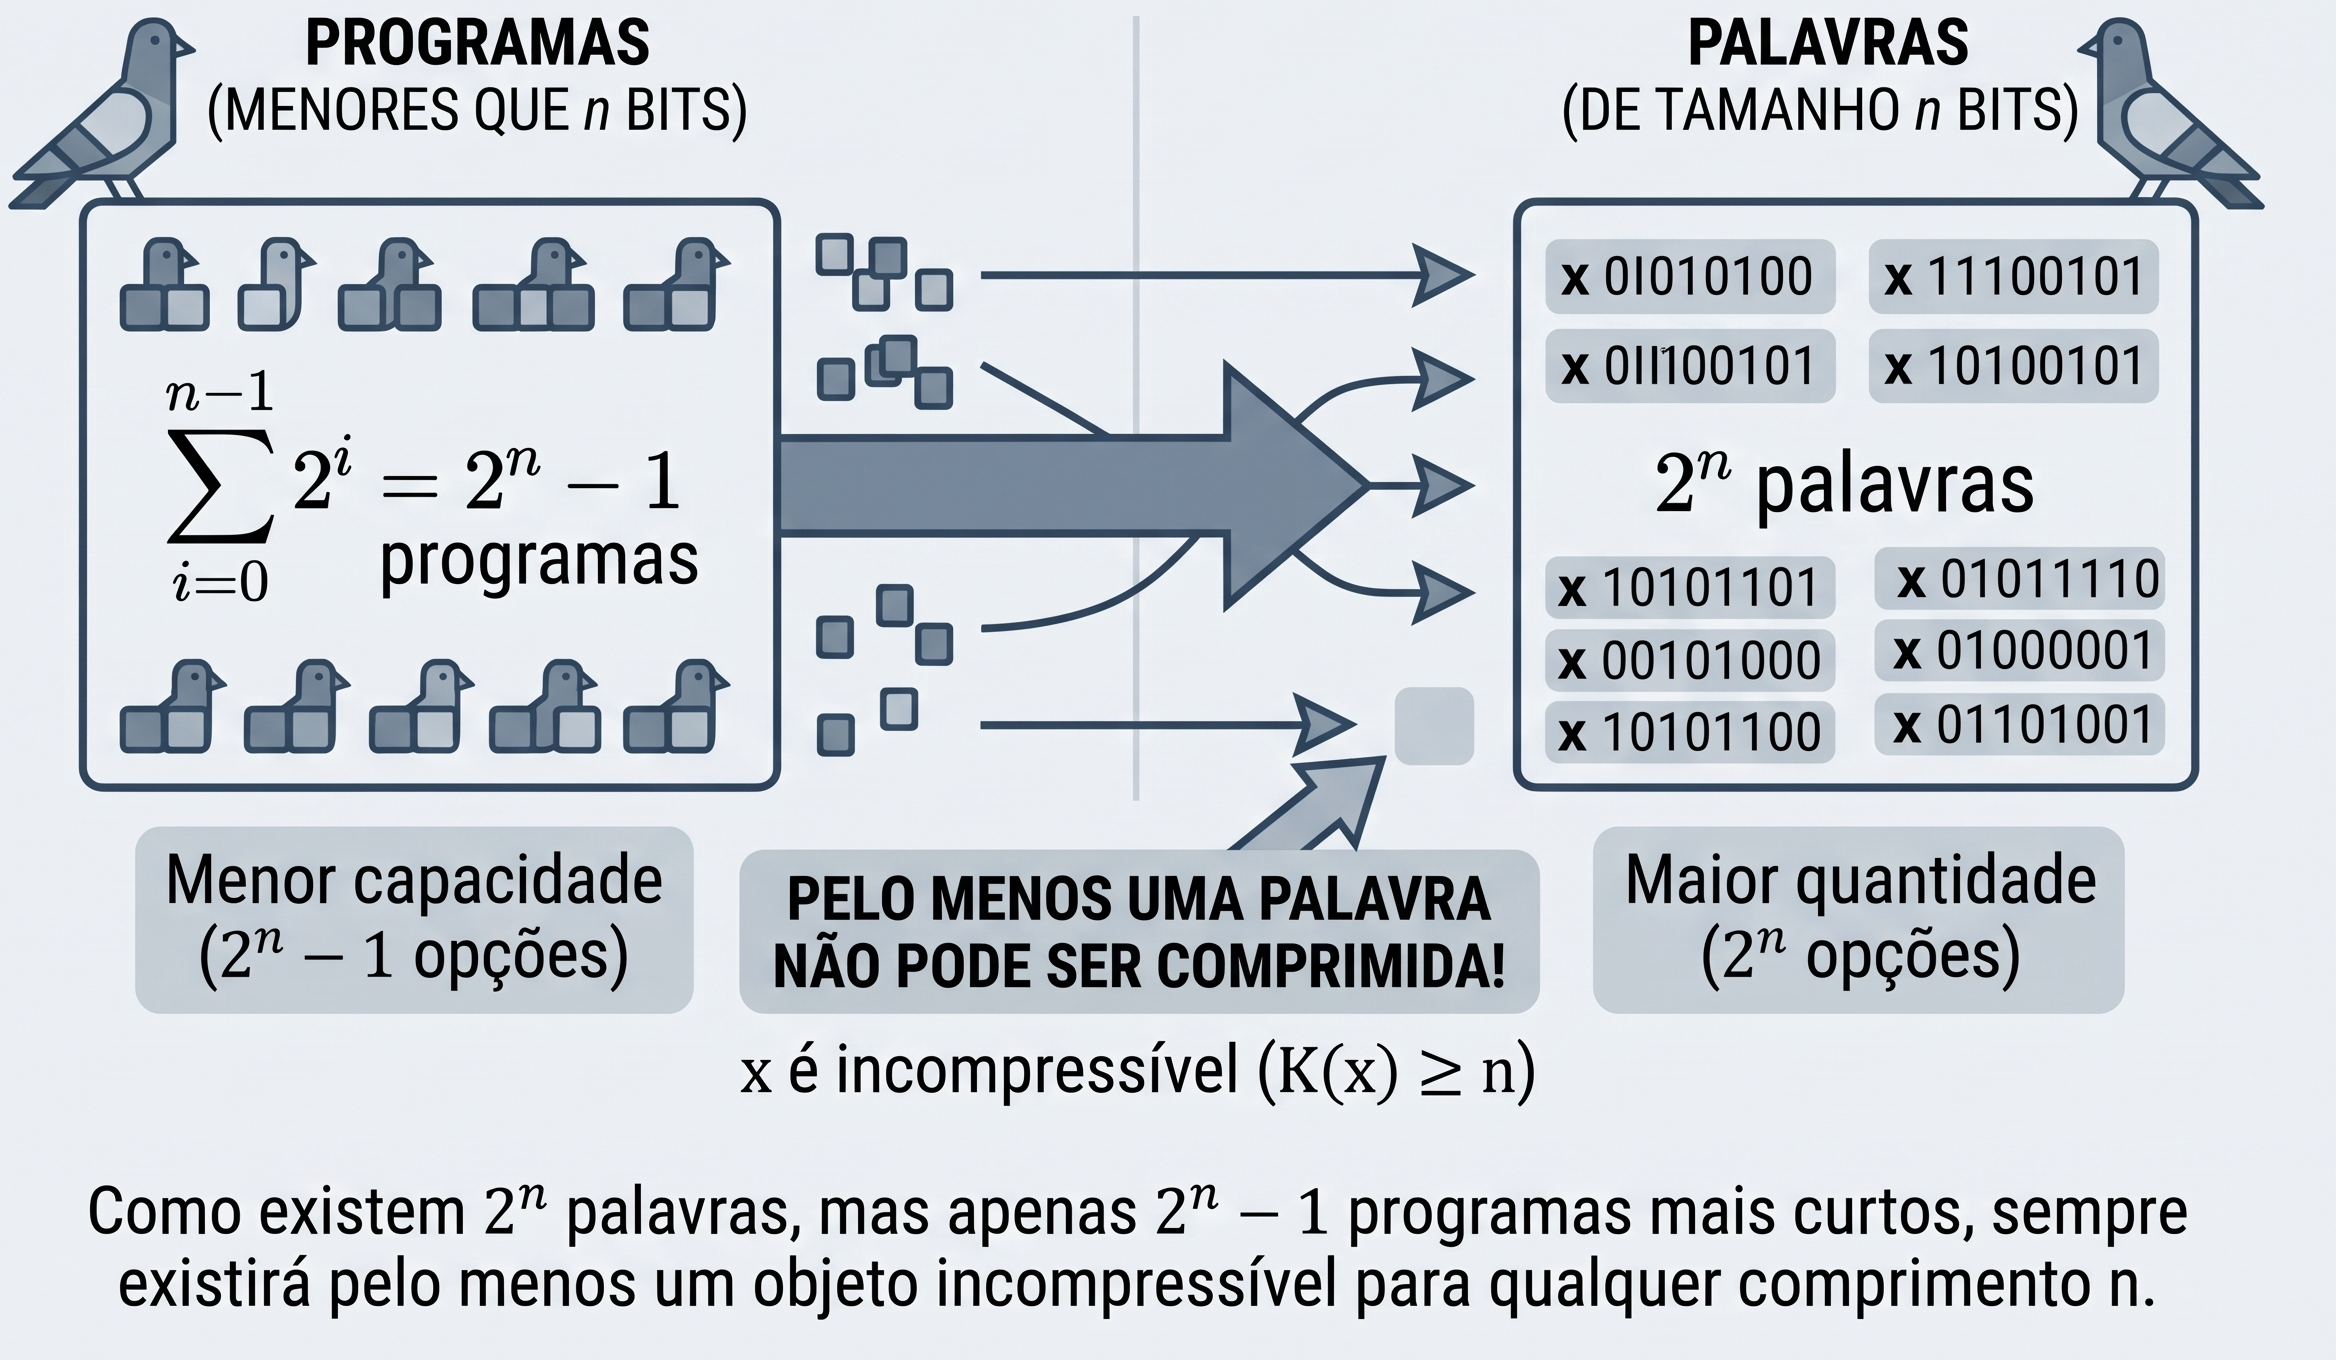
\includegraphics[width=0.95\textwidth]{figures/casa_pombos_definition.jpeg}
        \caption{\footnotesize{A violação do Princípio da Casa dos Pombos em relação à Complexidade de Kolmogorov.}}
        \label{fig:casa_pombos_definition}
    \end{figure}
\end{frame}

\begin{frame}{A Violação do Princípio em Strings $2^n$, sendo $n=4$}
\vspace{1mm}

\begin{figure}
    \centering
    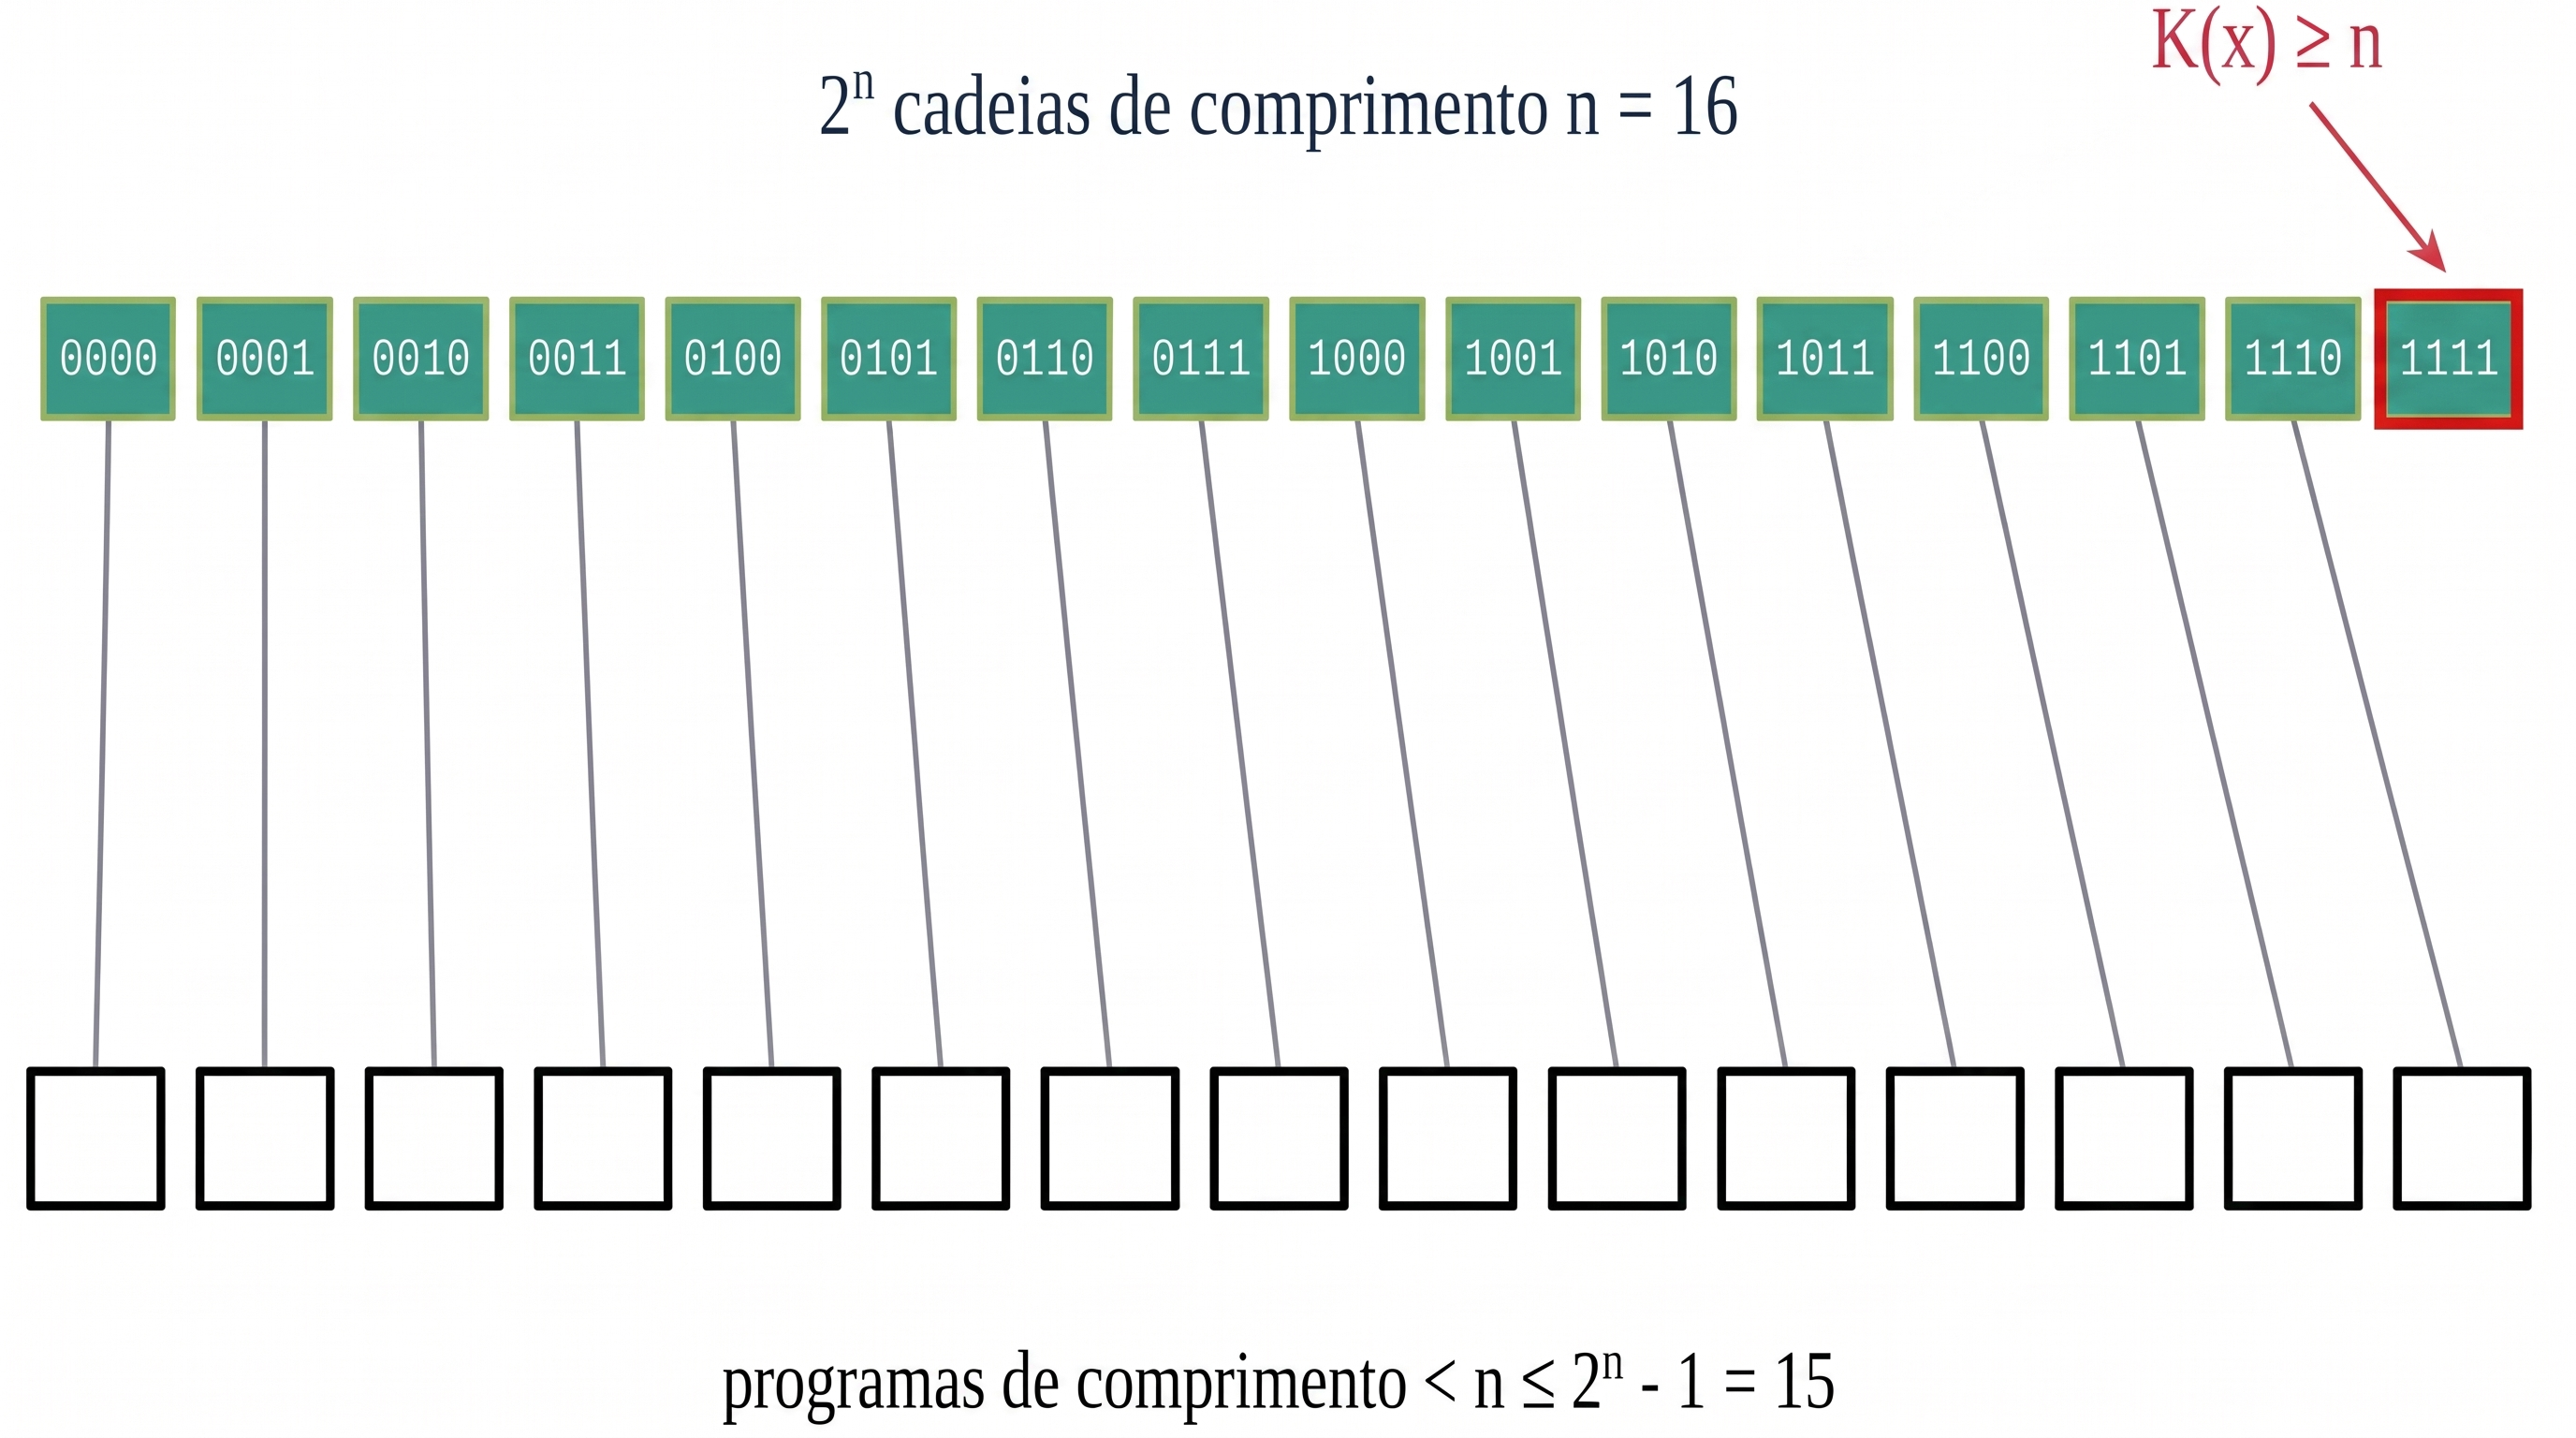
\includegraphics[width=0.93\textwidth]{figures/casa_pombos_example.jpeg}
    \caption{\footnotesize{A violação do Princípio da Casa dos Pombos em relação à Complexidade de Kolmogorov para uma string de $n = 4$.}}
    \label{fig:casa_pombos_example}
\end{figure}
\end{frame}

\begin{frame}{Limites Assintóticos e a Dualidade dos Primos}
    \small
    \begin{itemize}
        \item $p_m$: o $m$-ésimo primo ($p_1 = 2, p_2 = 3, \dots$);\quad $\pi(n) = |\{p \le n : p \text{ primo}\}|$;
        \item Limitar $p_m$ por \textbf{cima} equivale a limitar $\pi(n)$ por \textbf{baixo}: se $p_m$ não cresce rápido demais, há um número mínimo de primos em $[1, n]$.
    \end{itemize}
    \begin{figure}
        \centering
        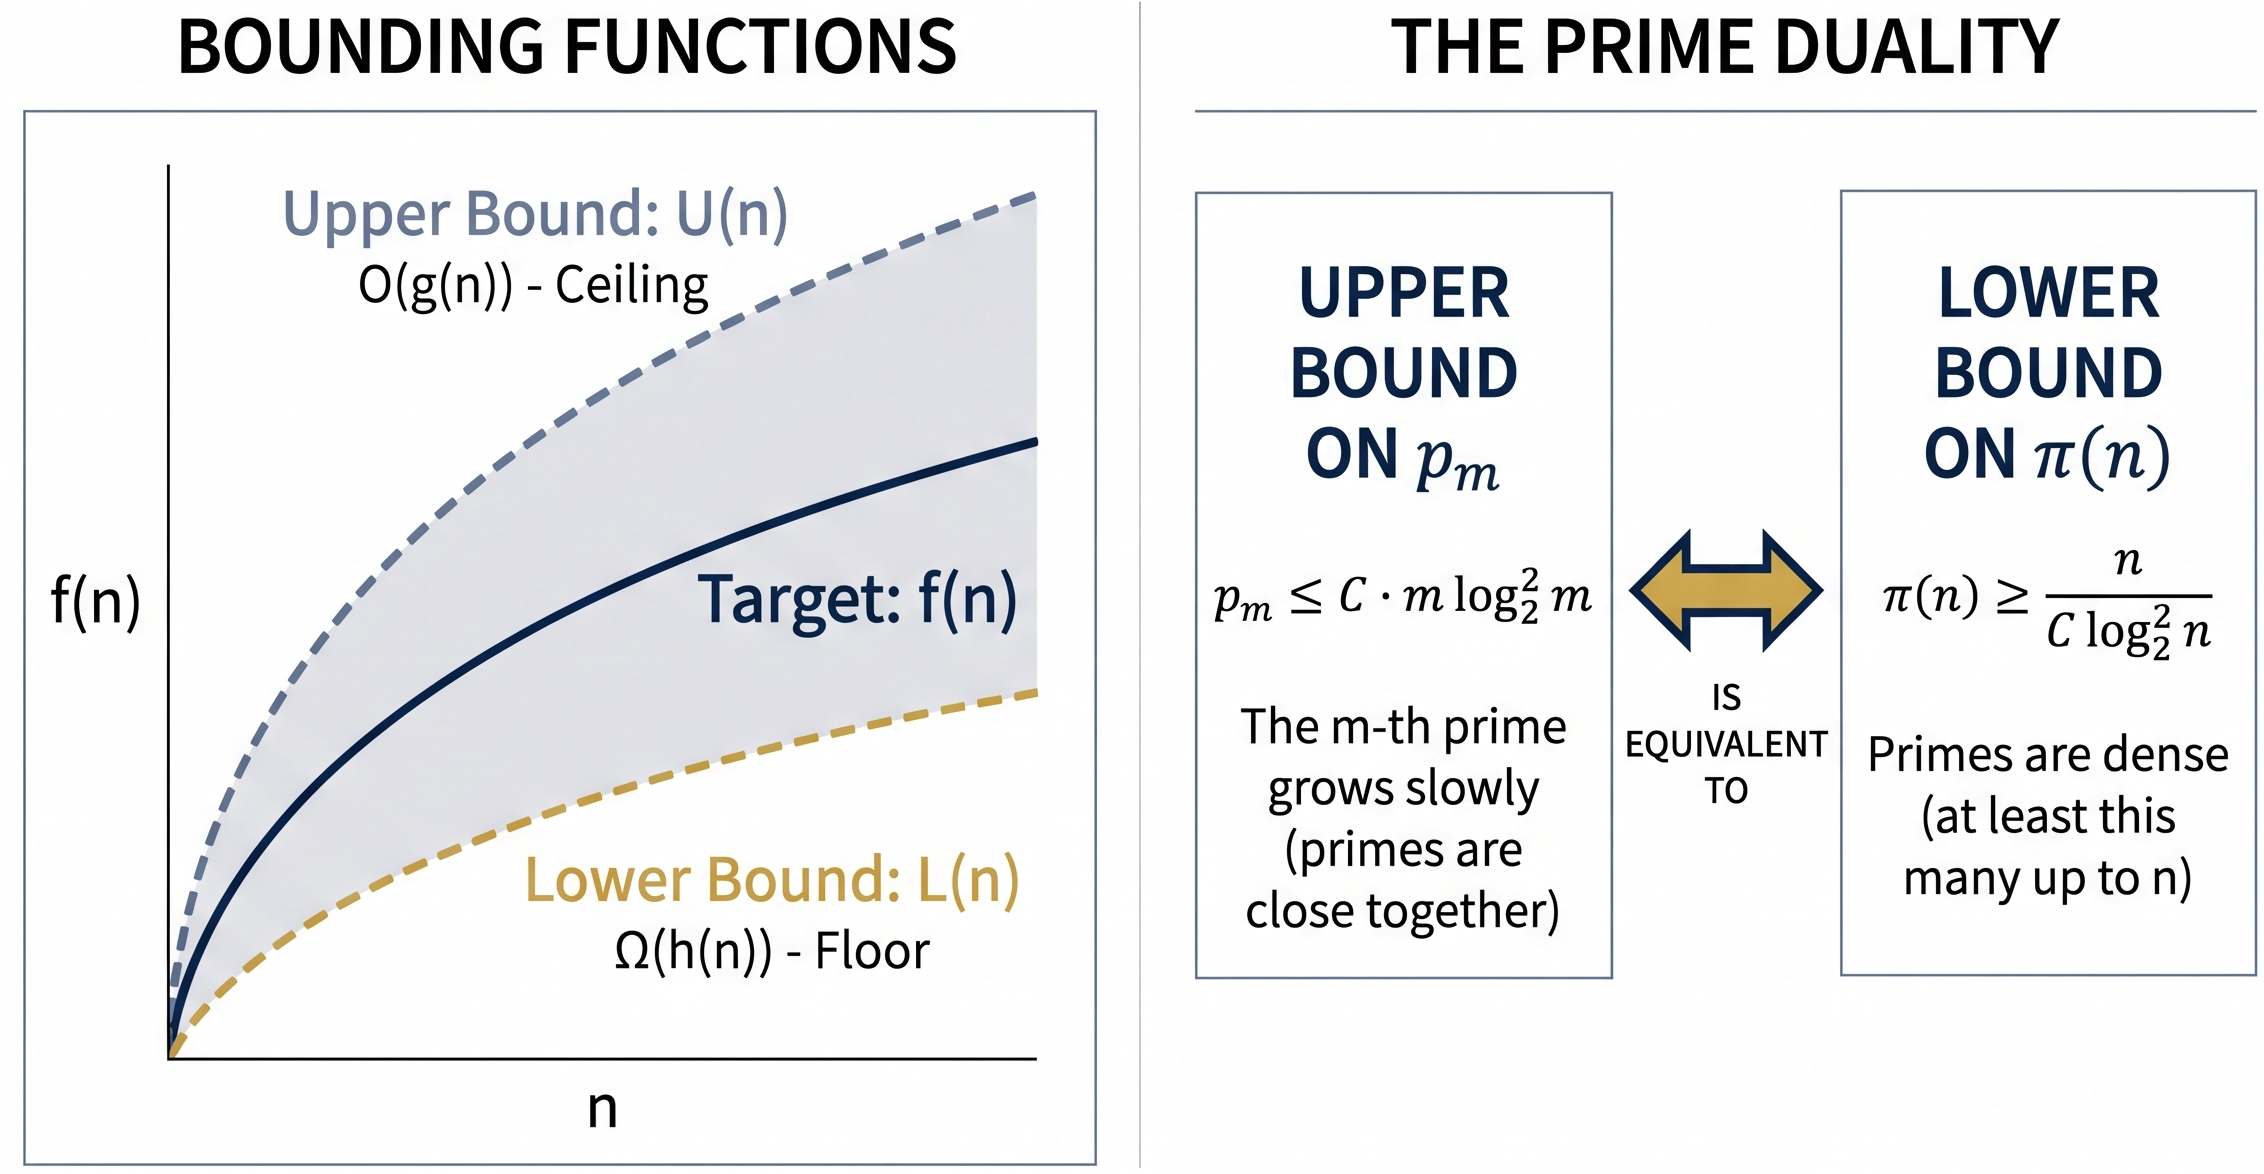
\includegraphics[width=0.86\textwidth]{figures/prime_duality.jpeg}
        \caption{\footnotesize{Cotas superiores ($\mathcal{O}$, teto) e inferiores ($\Omega$, piso), e a dualidade entre $p_m$ e $\pi(n)$.}}
        \label{fig:prime_duality}
    \end{figure}
\end{frame}

\begin{frame}{PNT Clássico vs. Teorema Fraco dos Primos}
    \begin{itemize}
        \item \textbf{\textit{Prime Number Theorem} (PNT) Clássico} (Hadamard e de la Vallée Poussin, 1896): exige análise complexa (zeros de $\zeta(s)$), o que torna sua formalização muito pesada \cite{apostol1976introduction, avigad2007formalPNT}:
        \begin{equation*}
            \pi(n) \sim \frac{n}{\ln n} \quad \Longleftrightarrow \quad p_m \sim m \ln m.
        \end{equation*}
        \item \textbf{Teorema Fraco dos Primos (\textit{Weak PNT})}: obtido apenas com matemática discreta e incompressibilidade \cite{schoning1998kolmogorov}:
        \begin{equation*}
            \pi(n) \ge \frac{n}{C (\log_2 n)^2} \quad \Longleftrightarrow \quad p_m \le C \cdot m (\log_2 m)^2.
        \end{equation*}
        \item \textbf{Por que ``fraco''?}
        \begin{enumerate}
            \item Desigualdade a menos de uma constante $C$, e não igualdade assintótica;
            \item Um fator extra de $\log_2 n$ no denominador, que corresponde \textbf{exatamente ao custo em bits do cabeçalho livre de prefixo} usado para separar $m$ de $k = n/p_m$ na fita binária.
        \end{enumerate}
    \end{itemize}
\end{frame}

\begin{frame}{PNT Clássico vs. Teorema Fraco dos Primos}
    \begin{figure}
        \centering
        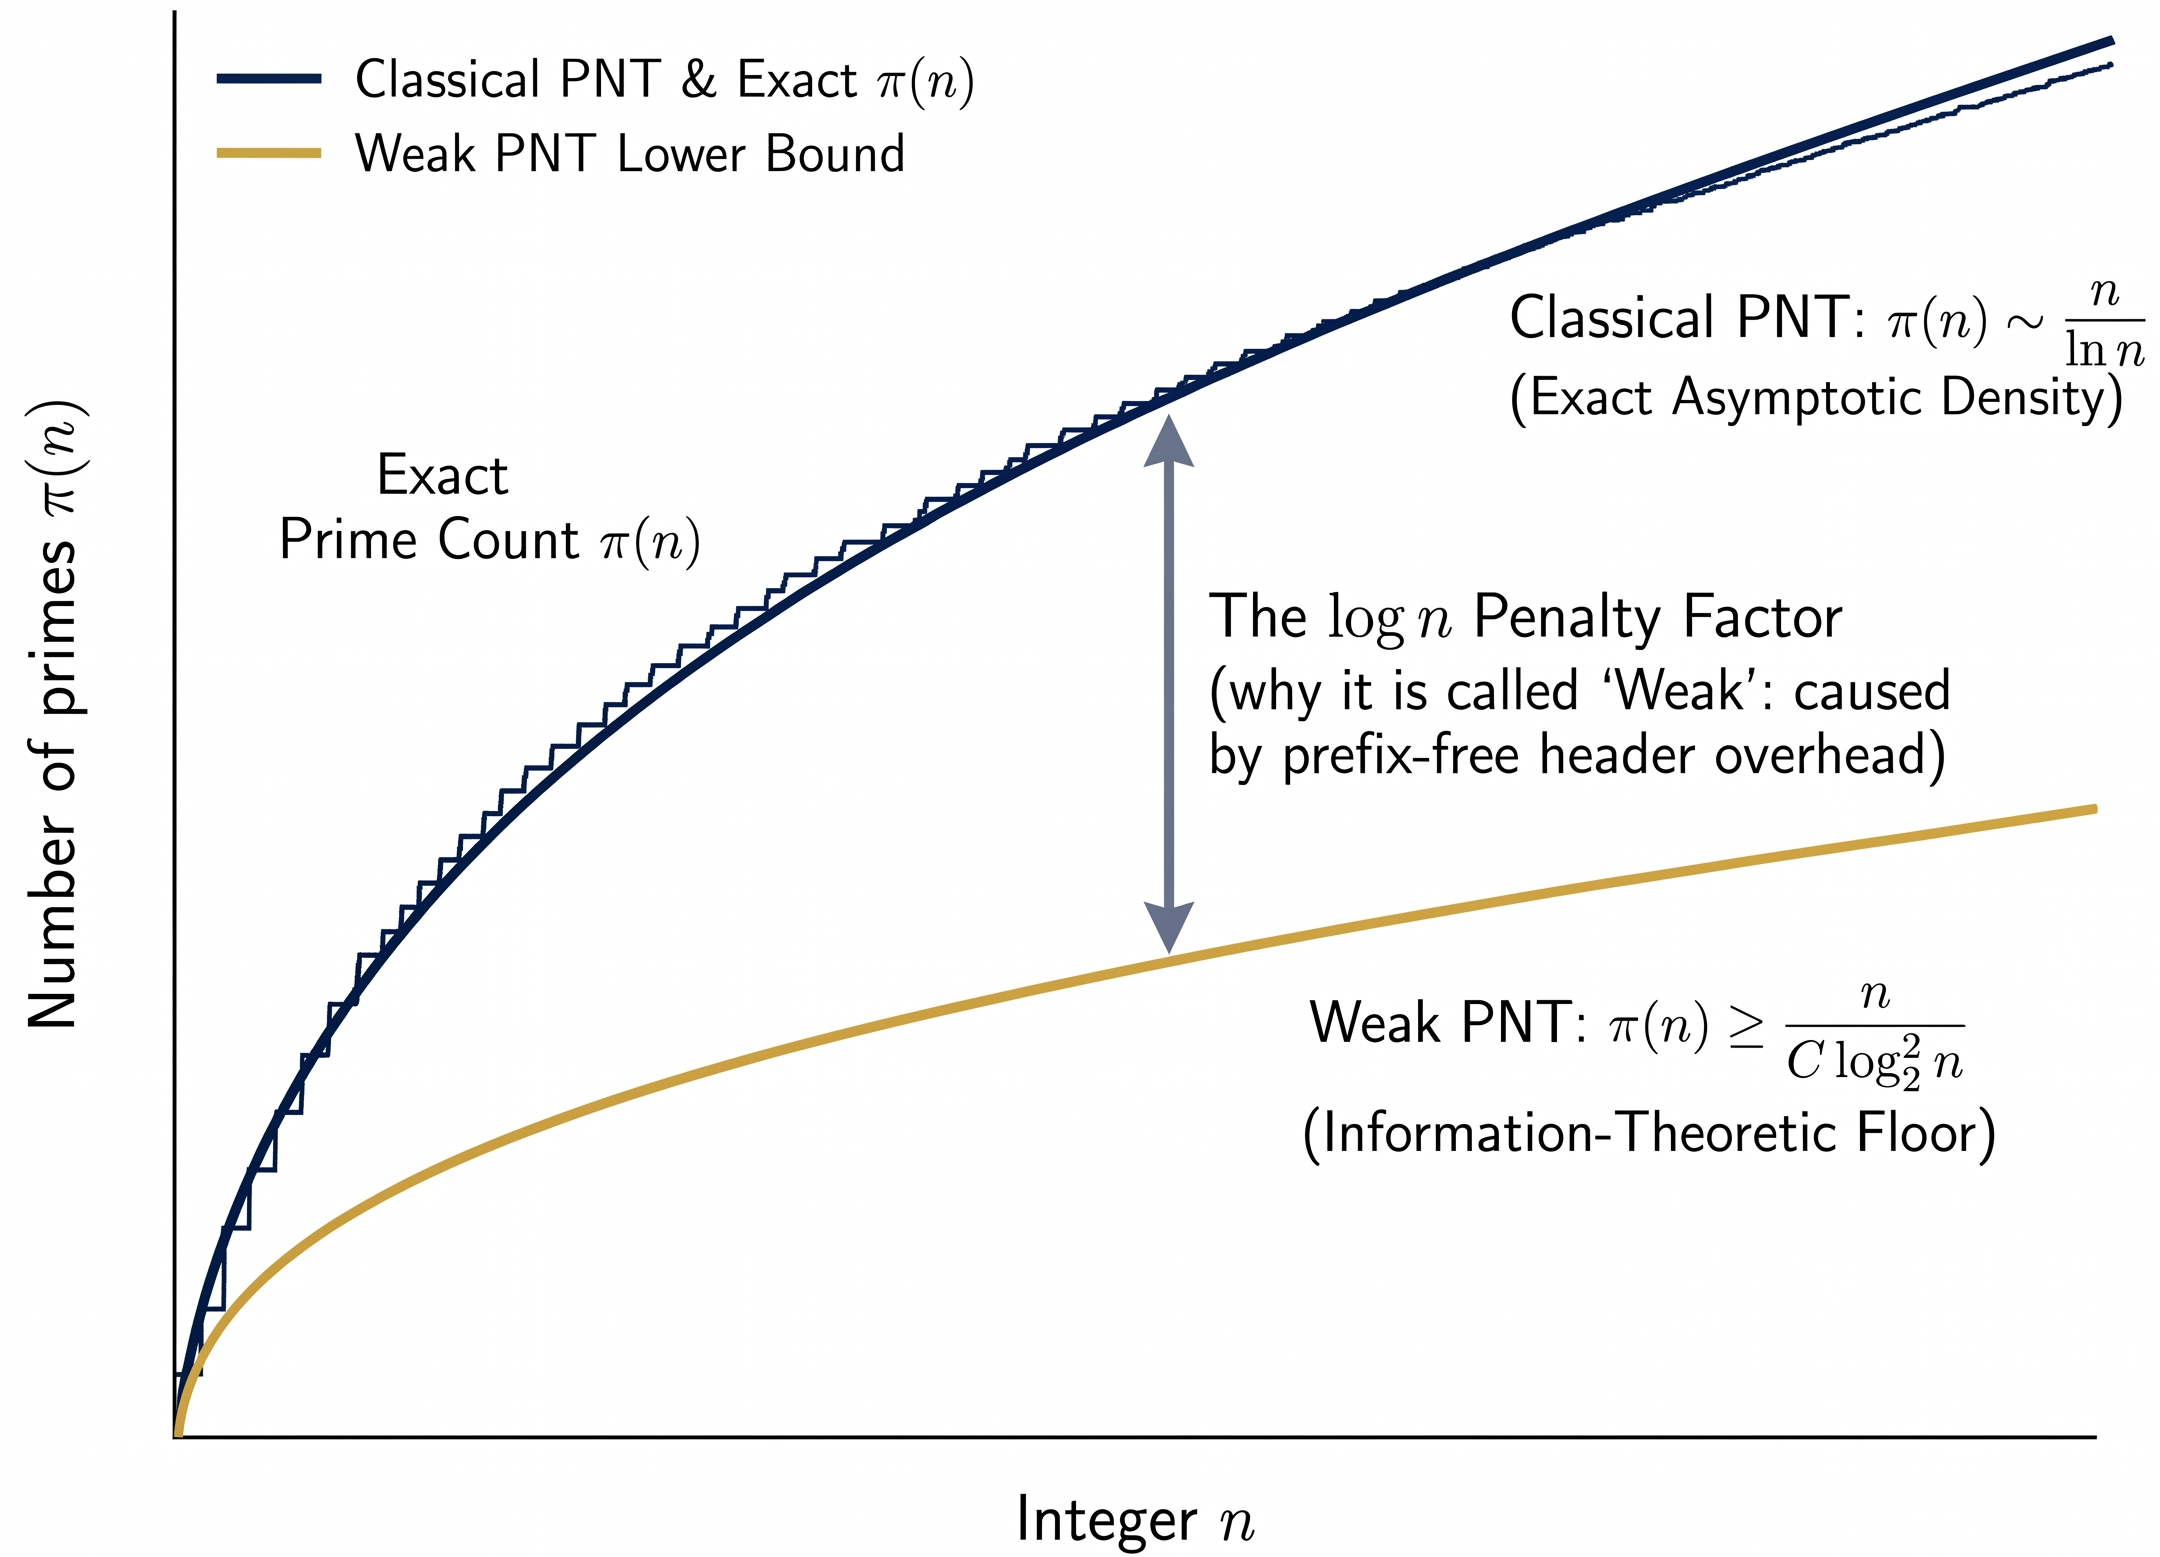
\includegraphics[height=0.66\textheight]{figures/weak_pnt.jpeg}
        \caption{\footnotesize{A contagem exata $\pi(n)$ e o PNT clássico (azul) vs. o piso do Weak PNT (dourado). A distância entre as curvas (fator $\log_2 n$) é o custo do cabeçalho livre de prefixo.}}
        \label{fig:weak_pnt}
    \end{figure}
\end{frame}

\begin{frame}{O Método da Incompressibilidade}
    \small
    \begin{itemize}
        \item Para toda string $x$ reconstruível a partir de uma codificação $E(x)$ por um decodificador fixo de $c$ bits: $K(x) \le |E(x)| + c$;
        \item Pela Casa dos Pombos, para todo $\ell$ existe $w \in \{0,1\}^\ell$ incompressível: $K(w) \ge |w|$.
    \end{itemize}
    \begin{tcolorbox}[pucbox, title=Motor do Método da Incompressibilidade]
        \begin{equation*}
            |w| \;\le\; K(w) \;\le\; |E(w)| + c
        \end{equation*}
        \footnotesize{Nenhuma codificação sem perdas $E$ comprime uma string incompressível em mais de $c$ bits.}
    \end{tcolorbox}
    \begin{enumerate}
        \item Tome $n$ incompressível e fatore-o como $n = p_m \cdot k$, sendo $p_m$ um fator primo;
        \item O par $\langle m, k \rangle$ descreve $n$ completamente, e $\text{bin}(k)$ economiza $\approx \log_2 p_m$ bits;
        \item Se os primos fossem escassos, o índice $m$ seria pequeno e $\langle m, k\rangle$ comprimiria $n$, \textbf{uma contradição}. Logo, $p_m$ não pode crescer rápido demais.
    \end{enumerate}
\end{frame}

\section[Problema]{Problema de Pesquisa}

\begin{frame}{Problema de Pesquisa: Do Esboço à Prova Mecânica}
\small
\begin{itemize}
    \item Nos livros-texto, o método da incompressibilidade aparece como \textbf{esboço semiformal} (Exercícios 9.1--9.5 de \citeonline{schoning1998kolmogorov}), deixando passos críticos implícitos:
    \begin{enumerate}
        \item Supõe-se que os bits de $m$ e de $k$ podem ser ``colados'' na fita \textbf{sem perda de informação};
        \item Usam-se identidades reais, como $\log_2(n/p) = \log_2 n - \log_2 p$, que \textbf{não valem} para logaritmos inteiros $\lfloor \log_2 \cdot \rfloor$ sobre $\mathbb{N}$.
    \end{enumerate}
    \medskip
    \item As primitivas necessárias estão em \textbf{duas bibliotecas distintas do Lean 4:}
    \begin{itemize}
        \item \textbf{Mathlib} \cite{mathlib2020}: primos, \texttt{Nat.nth}, \texttt{Nat.log}, mas \textbf{nenhuma} noção de complexidade de Kolmogorov;
        \item \textbf{Complexitylib} \cite{complexitylib2026} (\texttt{Cslib.Kolmogorov}): complexidade abstrata sobre strings, mas \textbf{sem} codificações aritméticas nem códigos autodelimitados.
    \end{itemize}
\end{itemize}
\end{frame}

\begin{frame}{Obstáculos para Integração das Bibliotecas}
\begin{enumerate}
    \item \textbf{Injetividade Dinâmica sobre Palavras Binárias:} uma palavra de tamanho variável \texttt{BinWord := List Bool} deve ser decodificada unicamente por uma hierarquia de códigos autodelimitados, sem erros de fronteira nem \textit{lookahead} durante a indução estrutural;
    \medskip
    \item \textbf{Estimativas Inteiras Discretas e Exatas:} as provas exigem desigualdades exatas sobre $\mathbb{N}$, como a superaditividade
    \begin{equation*}
        \lfloor\log_2 p\rfloor + \lfloor\log_2 k\rfloor \le \lfloor\log_2 (p\cdot k)\rfloor,
    \end{equation*}
    para que os bits do quociente se cancelem sem aproximações reais;
    \medskip
    \item \textbf{Não-Vacuidade Formal:} a hipótese de incompressibilidade (\texttt{h\_incomp}) deve ser satisfazível, para que os teoremas não sejam vacuamente verdadeiros.
\end{enumerate}
\end{frame}

\begin{frame}{O Propósito da Codificação Autodelimitada}
    \begin{figure}
        \centering
        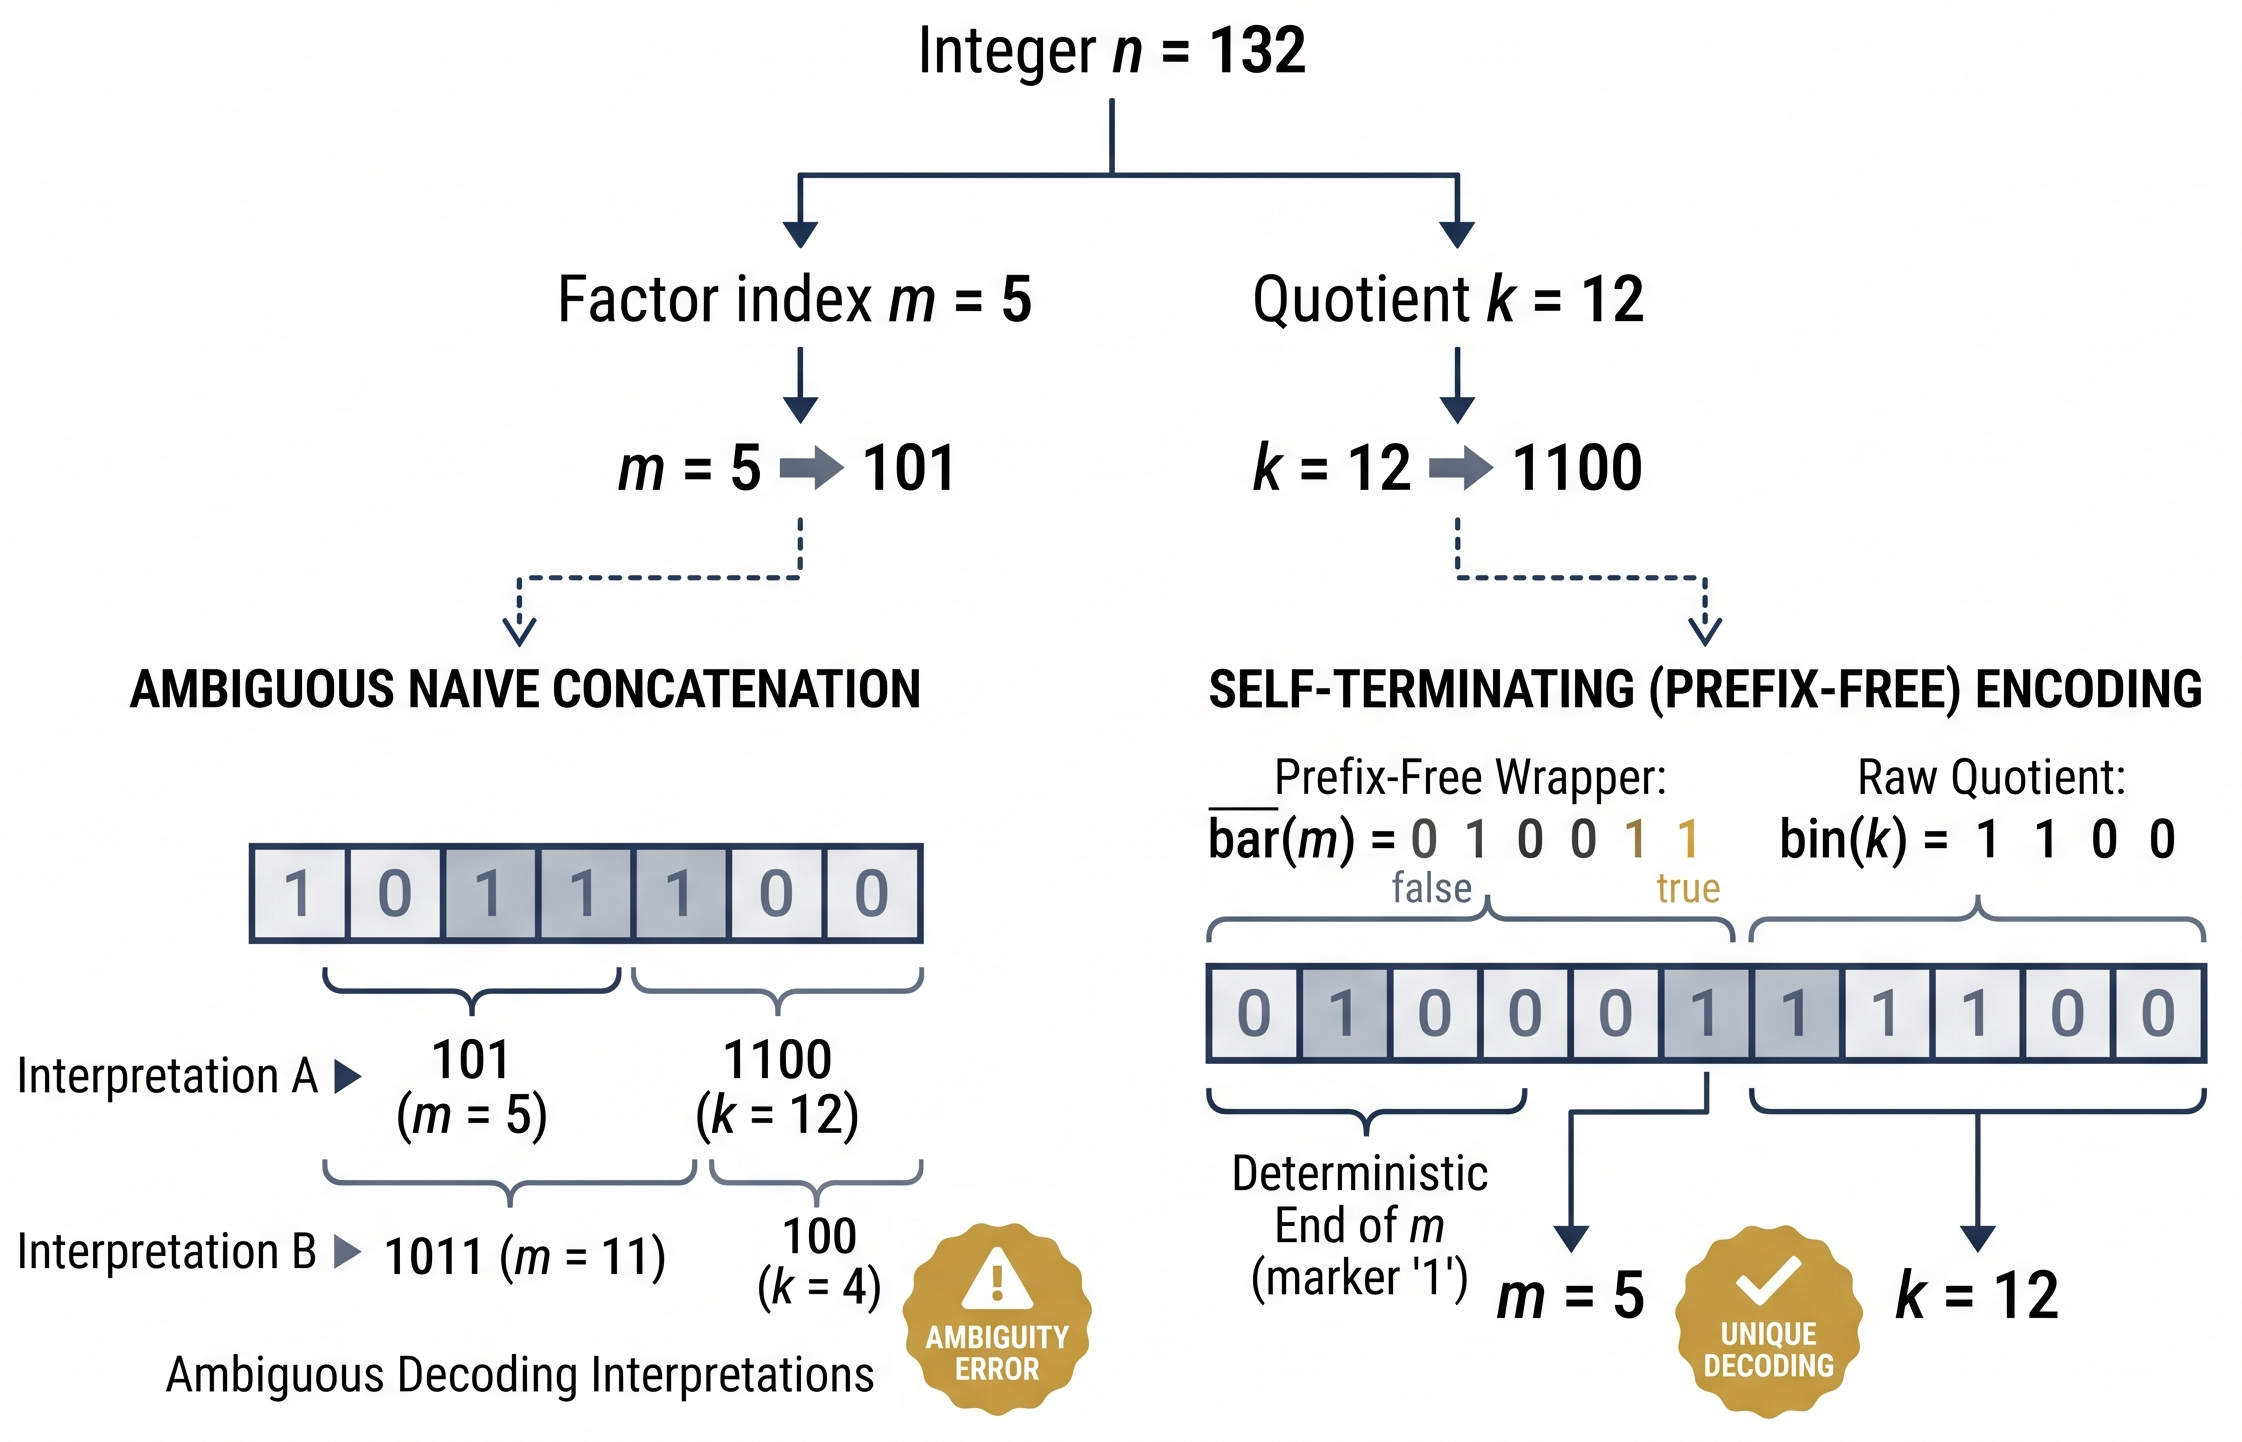
\includegraphics[height=0.66\textheight]{figures/prefix-free.jpeg}
        \caption{\footnotesize{Para $n = 132 = p_5 \cdot 12$, a concatenação ingênua \texttt{1011100} admite duas leituras ($m=5, k=12$ ou $m=11, k=4$). O código autodelimitado $\overline{\text{bin}(m)}$ marca o fim de $m$ e garante decodificação única.}}
        \label{fig:prefix_free}
    \end{figure}
\end{frame}

\begin{frame}{Proposta de Arquitetura para a Formalização}
    \begin{figure}
    \centering
    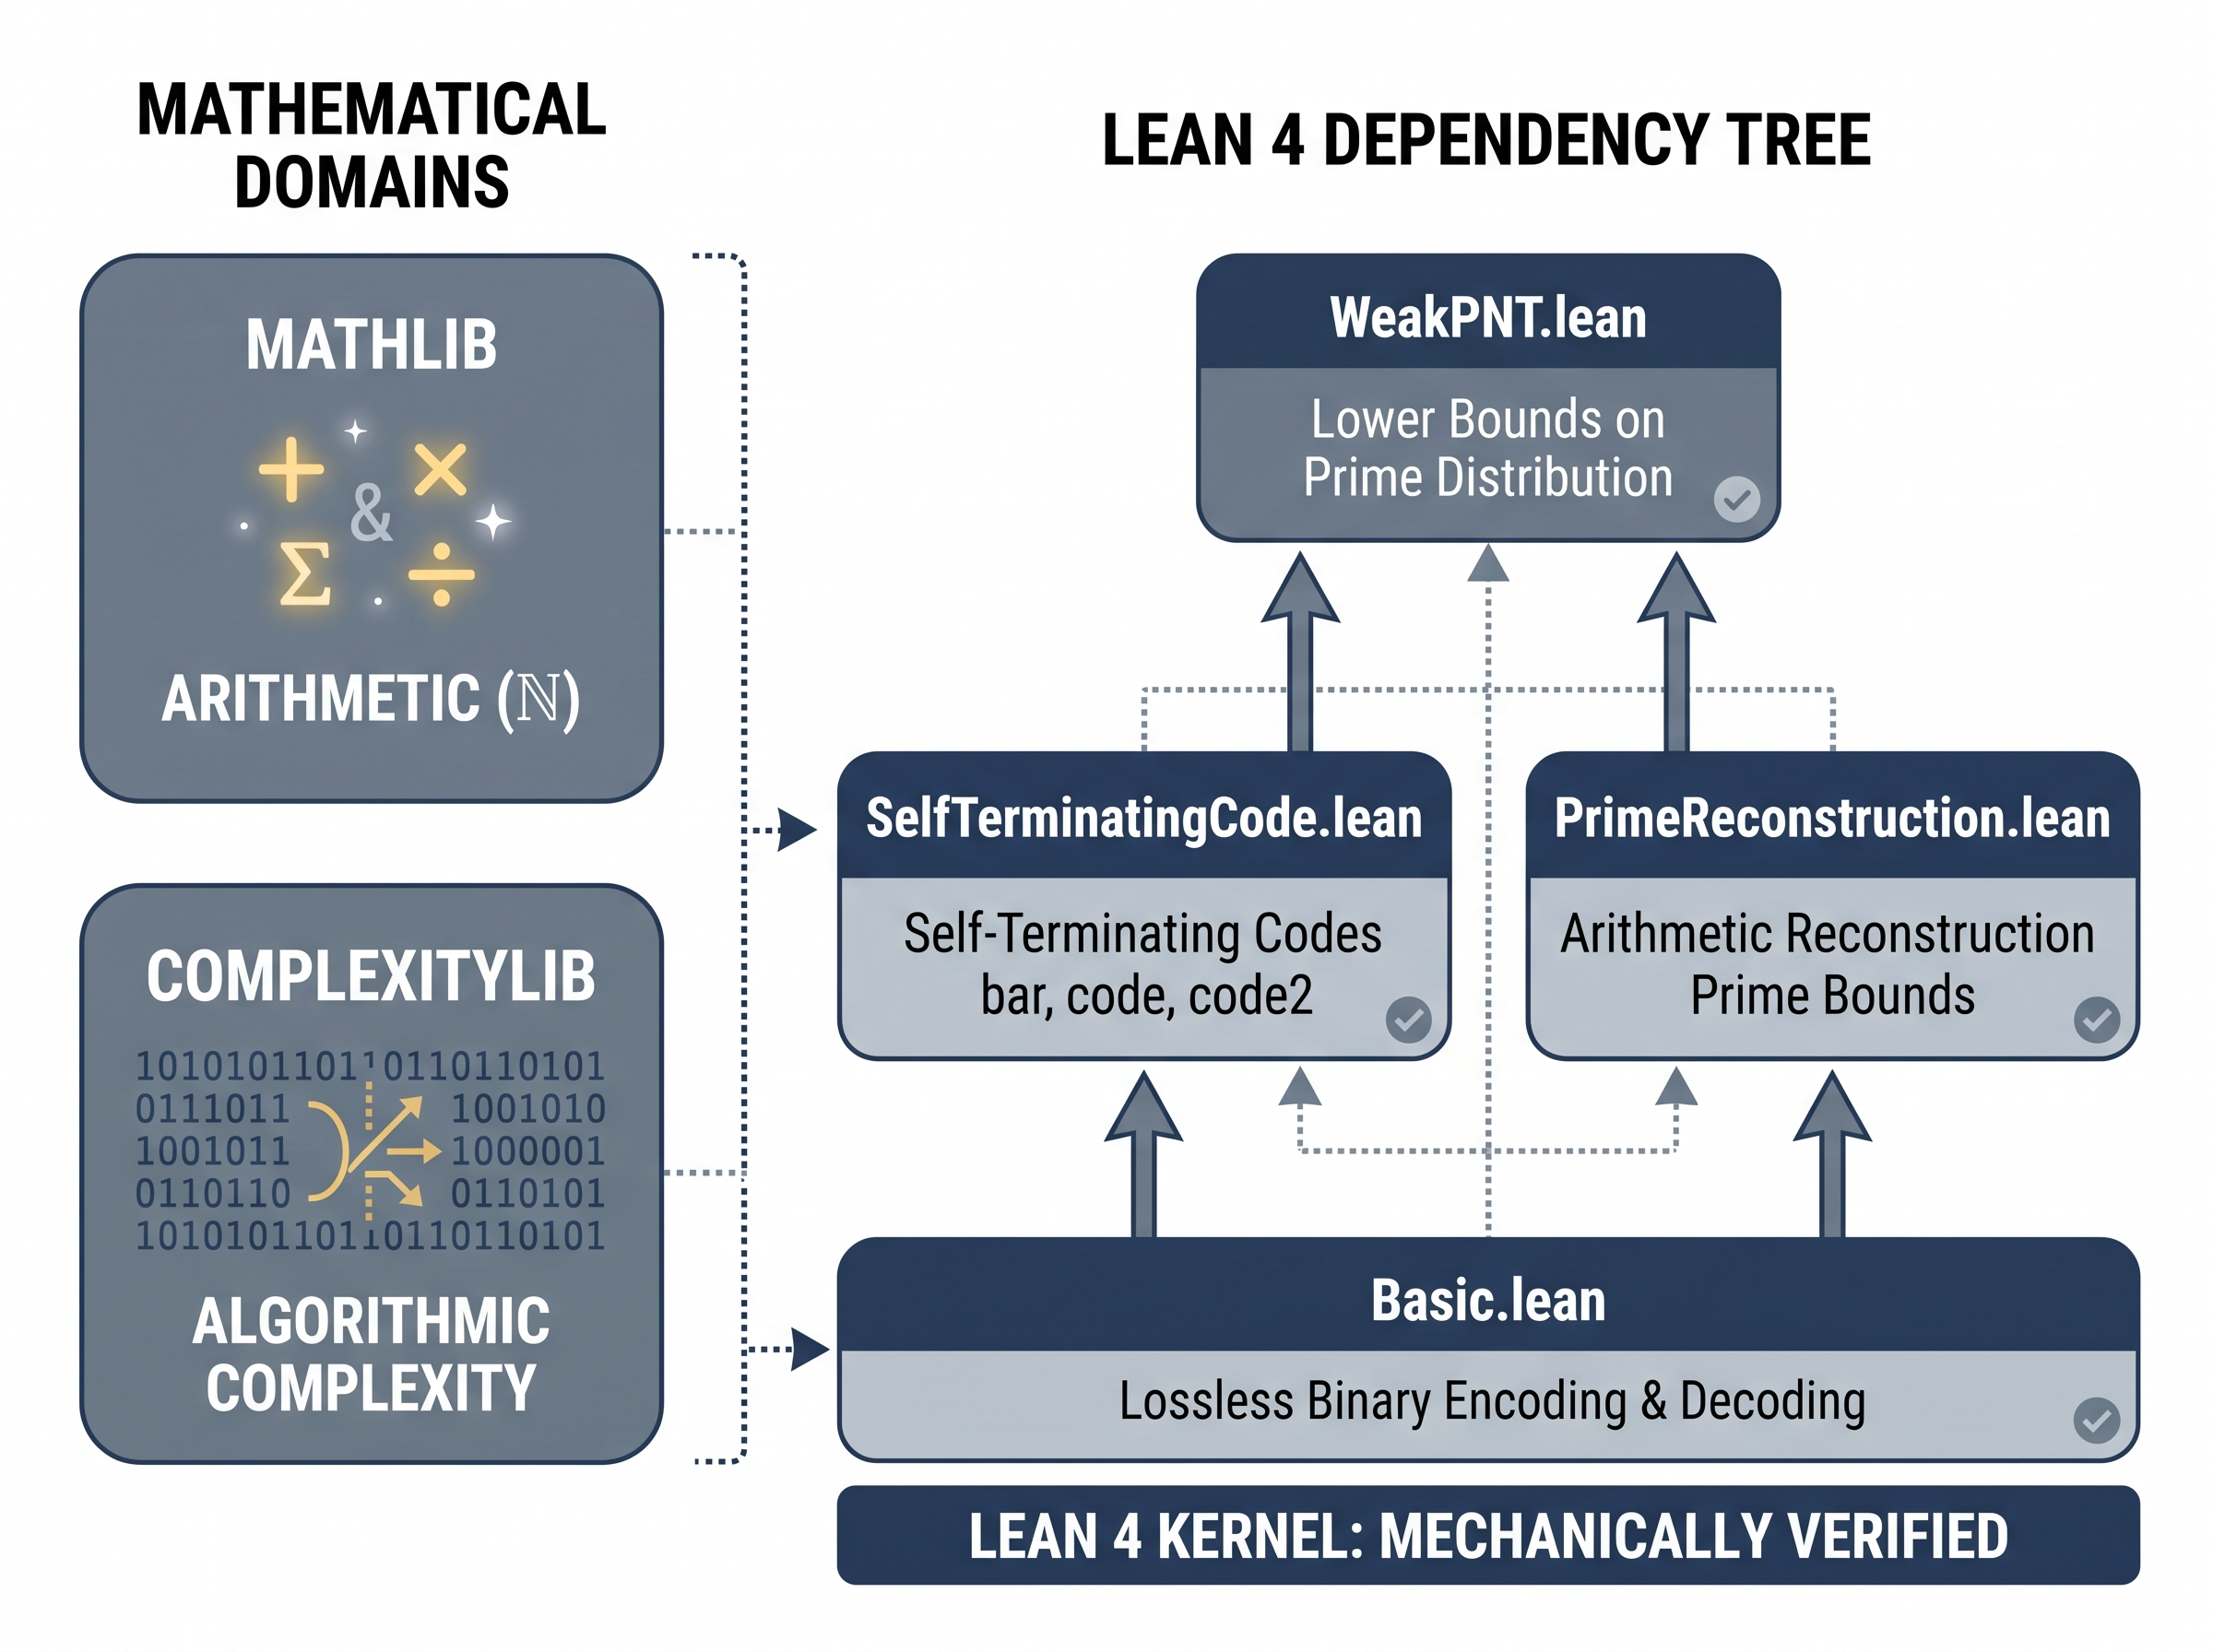
\includegraphics[height=0.66\textheight]{figures/objetive_filling_gap.jpeg}
    \caption{\footnotesize{À esquerda, os domínios matemáticos (\texttt{Mathlib} e \texttt{Complexitylib}). À direita, a árvore de dependências: \texttt{Basic.lean} sustenta os códigos autodelimitados e a reconstrução aritmética, que culminam em \texttt{WeakPNT.lean}.}}
    \label{fig:architecture}
    \end{figure}
\end{frame}

\begin{frame}{Problema de Pesquisa}
    \begin{tcolorbox}[pucbox, colframe=red!75!black, title=Problema Central de Pesquisa]
    Como transformar o argumento do método da incompressibilidade em uma \textbf{prova completa e mecanicamente verificada em Lean 4} (livre de \texttt{sorry}) do \textbf{Teorema Fraco dos Números Primos} e de seu \textbf{refinamento iterado}, construindo a ponte, hoje inexistente, entre a aritmética da \texttt{\textbf{Mathlib}} e a complexidade de Kolmogorov da \texttt{\textbf{Complexitylib}}?
    \end{tcolorbox}
\end{frame}

\section[Objetivos]{Objetivos Geral e Específicos}

\begin{frame}{Objetivo Geral}
    \begin{tcolorbox}[pucbox, title=Weak PNT Mecanicamente Verificado via Incompressibilidade]
        Provar em \textbf{Lean 4}, de forma completa, passo a passo e livre de \texttt{sorry}, o \textbf{Teorema Fraco dos Números Primos} pelo método da incompressibilidade de Kolmogorov, cobrindo os Exercícios 9.1--9.5 de \citeonline{schoning1998kolmogorov}:
        \begin{equation*}
            \pi(n) \ge \frac{n}{C\,(\log_2 n)^2} \quad\Longleftrightarrow\quad p_m \le C \cdot m\,(\log_2 m)^2,
        \end{equation*}
        bem como seu \textbf{refinamento iterado}, obtido comprimindo o cabeçalho livre de prefixo uma segunda vez:
        \begin{equation*}
            p_m = \mathcal{O}\big(m \log_2 m\,(\log_2\log_2 m)^2\big).
        \end{equation*}
    \end{tcolorbox}
\end{frame}

\begin{frame}{Objetivos Específicos I}
\begin{enumerate}
    \item \textbf{Ponte Aritmético-Informacional (\texttt{Basic.lean}):}
    \begin{itemize}
        \item Representar $n \in \mathbb{N}$ como \texttt{BinWord} (\texttt{bin}, little-endian via \texttt{Nat.bits}) com decodificador inverso à esquerda (\texttt{decodeBin}) e injetividade;
        \item Provar a identidade exata $|\text{bin}(n)| = \lfloor\log_2 n\rfloor + 1$ para $n > 0$;
        \item Conectar-se à complexidade \texttt{ecomplexity} (valores em \texttt{ENat}) da \texttt{Complexitylib}.
    \end{itemize}
    \medskip
    \item \textbf{Hierarquia de Códigos Autodelimitados (\texttt{SelfTerminatingCode.lean}):}
    \begin{itemize}
        \item Construir os códigos livres de prefixo elementar ($\overline{w}$), compacto ($\text{code}$) e iterado ($\text{code}_2$) por recursão total e sem \textit{lookahead};
        \item Provar a decodificação única de cada camada e suas cotas exatas de comprimento.
    \end{itemize}
\end{enumerate}
\end{frame}

\begin{frame}{Objetivos Específicos II}
\begin{enumerate}
    \setcounter{enumi}{2}
    \item \textbf{Infinitude e Redução Analítica (\texttt{InfinitudePrimes.lean}, \texttt{PrimeReconstruction.lean}):}
    \begin{itemize}
        \item Provar a infinitude dos primos por compressão da tupla de expoentes;
        \item Formalizar a reconstrução injetora $n = p_m \cdot k$ e a redução discreta de cotas de $p_m$ para cotas de $\pi(n)$.
    \end{itemize}
    \medskip
    \item \textbf{Weak PNT e Refinamento Iterado (\texttt{WeakPNT.lean}):}
    \begin{itemize}
        \item Provar a \textbf{Inequação Central de Balanço de Bits} $\lfloor\log_2 p_m\rfloor \le |\text{enc}_m| + c$;
        \item Derivar $\pi(n) = \Omega(n/\log_2^2 n)$ e $p_m = \mathcal{O}(m \log_2 m (\log_2\log_2 m)^2)$.
    \end{itemize}
    \medskip
    \item \textbf{Verificação Mecânica:} garantir zero \texttt{sorry}, demonstrar a não-vacuidade das hipóteses e isolar o pressuposto de computabilidade numa constante explícita $c$ (\texttt{h\_desc}).
\end{enumerate}
\end{frame}

\section{Resultados}

\begin{frame}{Visão Geral: Cinco Módulos Verificados sem \texttt{sorry}}
\footnotesize
\renewcommand{\arraystretch}{1.3}
\begin{table}
\centering
\resizebox{\textwidth}{!}{
\begin{tabular}{@{}lL{7.6cm}@{}}
\toprule
\textbf{Módulo} & \textbf{Resultados Principais Verificados} \\
\midrule
\texttt{Basic.lean} & \texttt{bin\_injective}, $|\text{bin}(n)| = \lfloor\log_2 n\rfloor + 1$, \texttt{exists\_incompressible\_word} \\
\texttt{SelfTerminatingCode.lean} & $|\overline{w}| = 2|w| + 1$; injetividade de \texttt{bar}, \texttt{code} e \texttt{code2}; cotas de comprimento \\
\texttt{InfinitudePrimes.lean} & Injetividade de \texttt{encodeExponents}; $p^e \mid n \Rightarrow e \le \lfloor\log_2 n\rfloor$; infinitude dos primos \\
\texttt{PrimeReconstruction.lean} & $p_m \cdot (n/p_m) = n$; injetividade de \texttt{encodePairCode}/\texttt{encodePairCode2}; redução analítica \\
\texttt{WeakPNT.lean} & Superaditividade de $\lfloor\log_2\rfloor$; Balanço de Bits; ponte exponencial; \textbf{Weak PNT}; cota iterada \\
\bottomrule
\end{tabular}
}
\caption{Módulos da formalização e seus principais teoremas.}
\end{table}
\end{frame}

\begin{frame}{Hierarquia de Códigos Autodelimitados}
    \begin{figure}
        \centering
        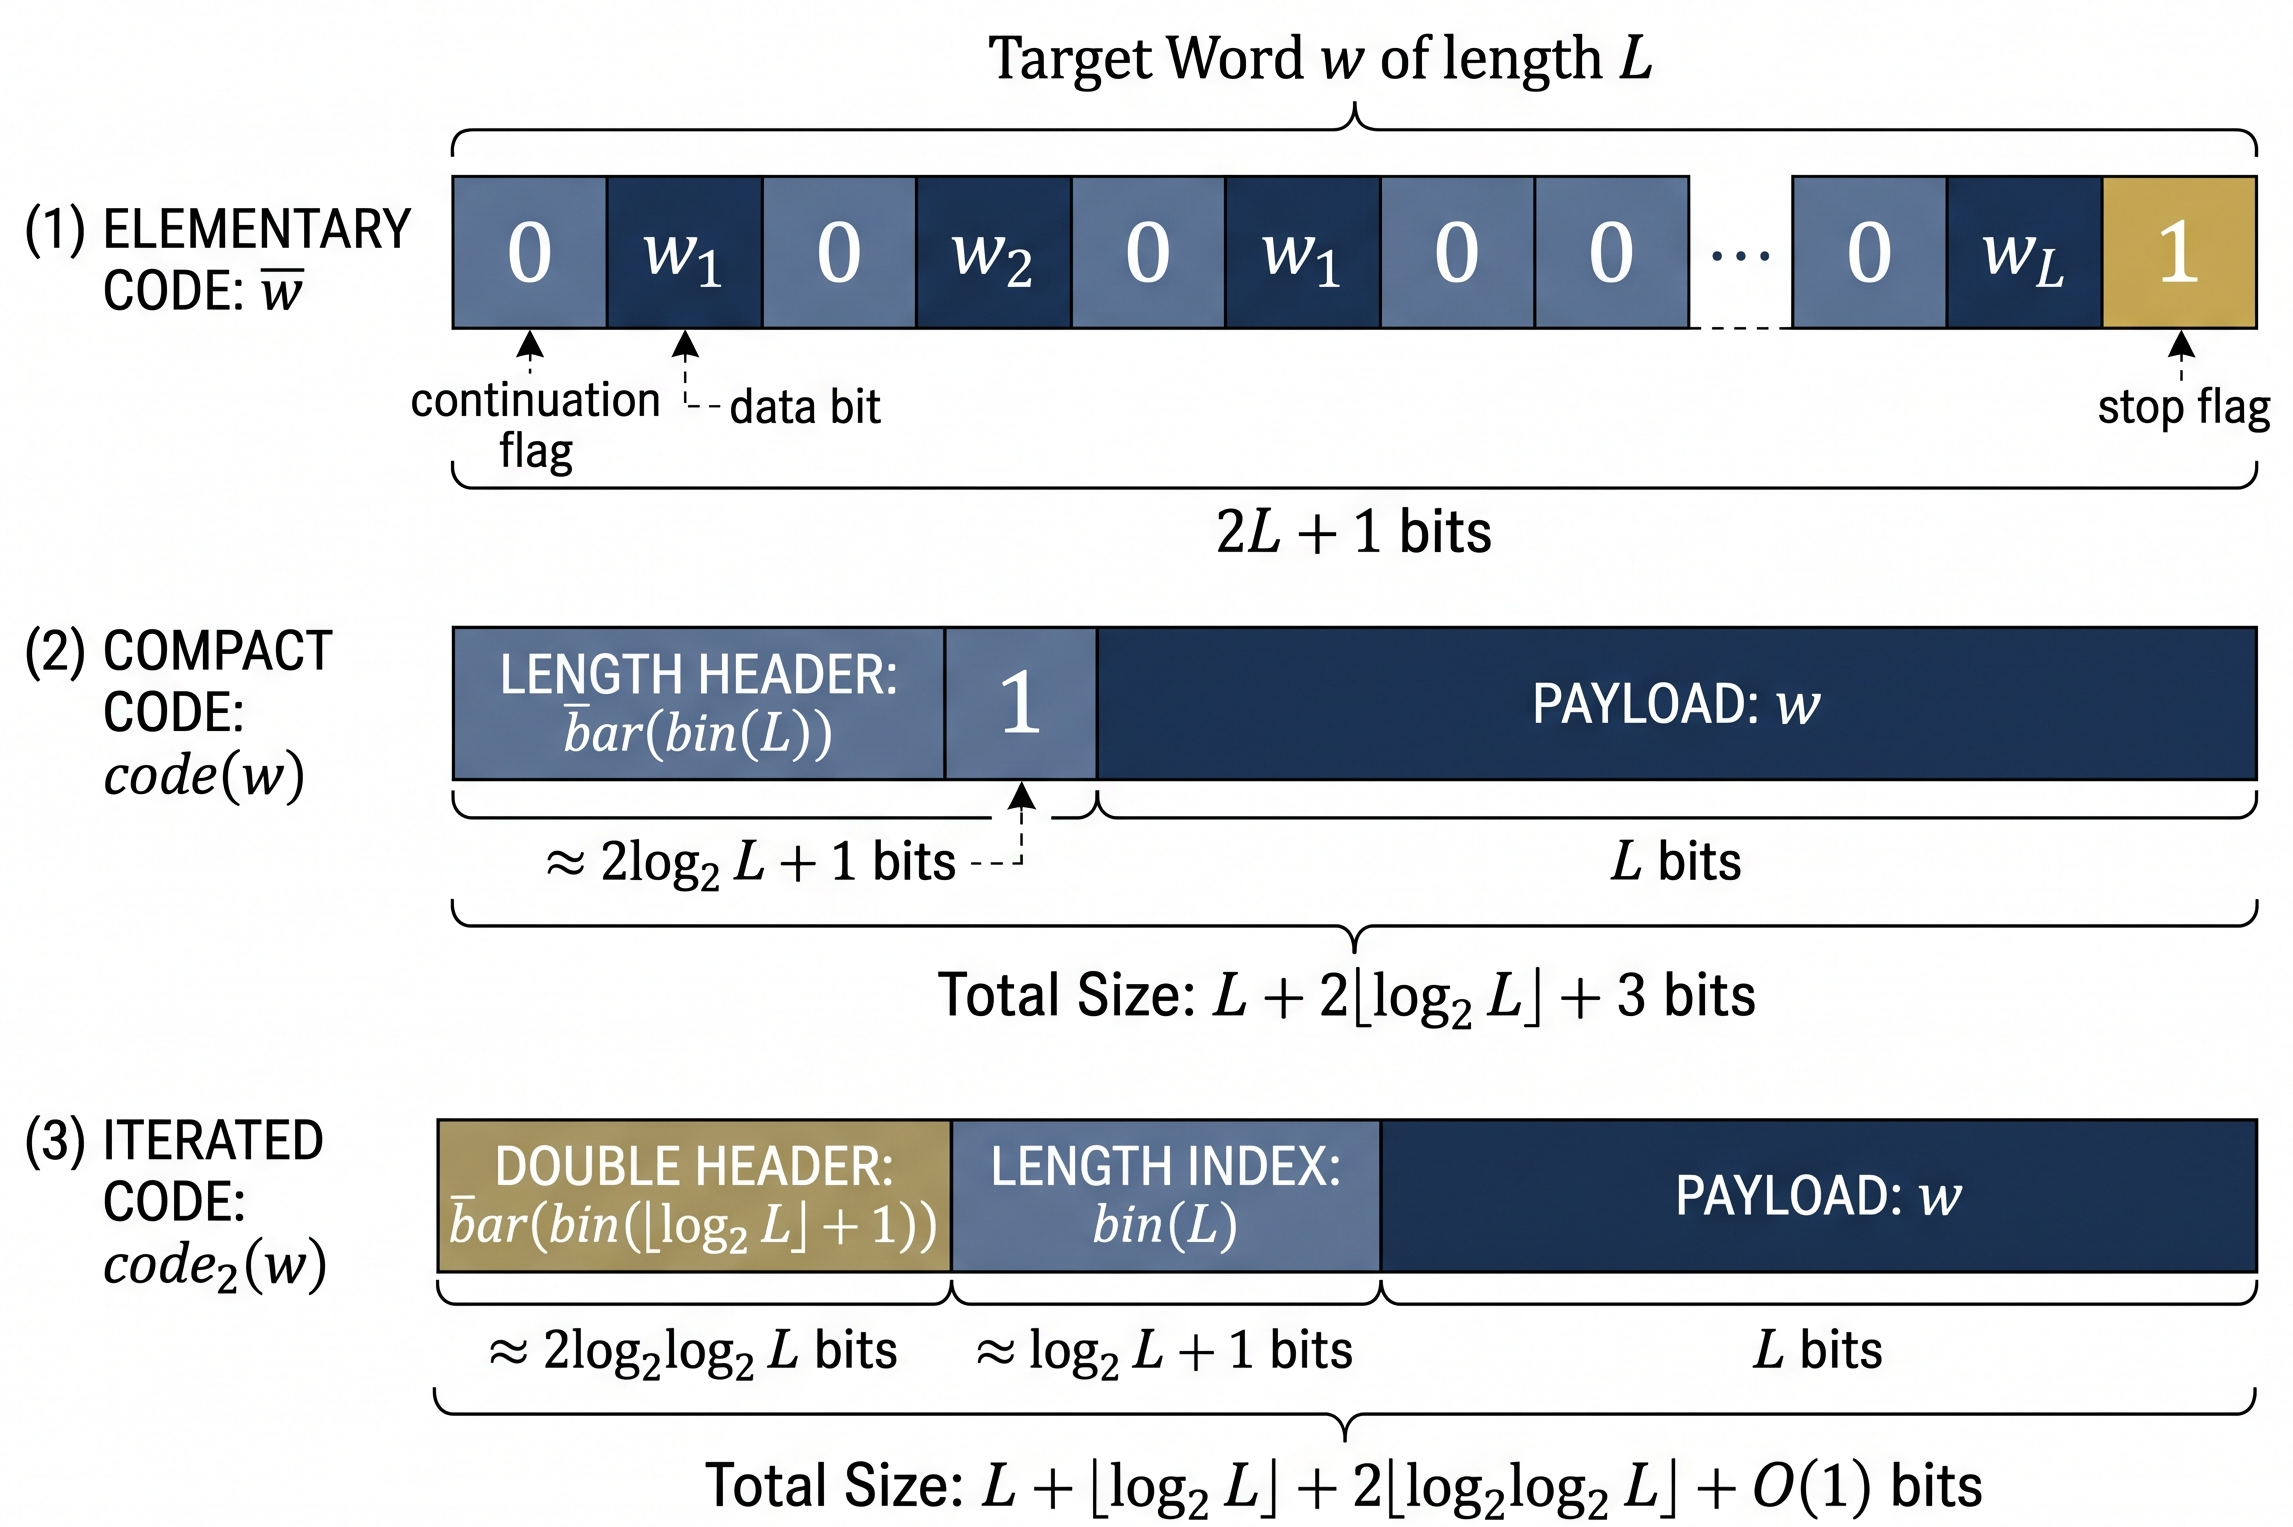
\includegraphics[height=0.66\textheight]{figures/hierarchy_of_self_terminating_codes.jpeg}
        \caption{\footnotesize{Layout de bits dos três códigos para uma palavra $w$ de tamanho $L$: elementar ($2L + 1$ bits), compacto ($L + 2\lfloor\log_2 L\rfloor + 3$) e iterado ($L + \lfloor\log_2 L\rfloor + 2\lfloor\log_2\log_2 L\rfloor + O(1)$).}}
        \label{fig:code_hierarchy}
    \end{figure}
\end{frame}

\begin{frame}[fragile]{Códigos Autodelimitados em Lean 4}
\small
Construção \textit{flag-prefixed}: cada bit é precedido pela flag de continuação \texttt{false} e a palavra termina com a flag de parada \texttt{true}. É \textbf{total} (inclusive em \texttt{[]}) e dispensa \textit{lookahead}.
\begin{lstlisting}[language=Lean4]
abbrev BinWord := List Bool

def bar (s : BinWord) : BinWord :=
  match s with
  | [] => [true]
  | b :: bs => false :: b :: bar bs

def code (w : BinWord) : BinWord :=
  bar (bin w.length) ++ w

def code2 (w : BinWord) : BinWord :=
  code (bin w.length) ++ w
\end{lstlisting}
\begin{itemize}
    \item $|\overline{w}| = 2|w| + 1$; \quad $|\text{code}(w)| \le |w| + 2\lfloor\log_2|w|\rfloor + 3$;
    \item $|\text{code}_2(w)| \le |w| + \lfloor\log_2|w|\rfloor + 2\lfloor\log_2(\lfloor\log_2|w|\rfloor + 1)\rfloor + 4$.
\end{itemize}
\end{frame}

\begin{frame}{Injetividade Livre de Prefixo Composicional}
    \begin{tcolorbox}[pucbox, title=Teorema (Injetividade Livre de Prefixo)]
        \small (\texttt{bar\_append\_inj}, \texttt{code\_append\_inj}, \texttt{code2\_append\_inj}) Para $C \in \{\text{bar}, \text{code}, \text{code}_2\}$ e quaisquer $w_1, w_2, v_1, v_2 \in \texttt{BinWord}$:
        \begin{equation*}
            C(w_1) \mathbin{+\!+} v_1 = C(w_2) \mathbin{+\!+} v_2 \implies w_1 = w_2 \;\wedge\; v_1 = v_2.
        \end{equation*}
    \end{tcolorbox}
    \small
    \begin{enumerate}
        \item \textbf{Camada base (\texttt{bar}):} indução estrutural em $w_1$; cabeças \texttt{true} $\neq$ \texttt{false} descartam casos impossíveis e a injetividade de construtores remove dois bits por vez;
        \item \textbf{Camada compacta (\texttt{code}):} \texttt{bar\_append\_inj} separa o cabeçalho; \texttt{bin\_injective} dá $|w_1| = |w_2|$; \texttt{List.append\_inj} separa $w_i$ de $v_i$, \textbf{sem nova indução};
        \item \textbf{Camada iterada (\texttt{code2}):} mesmo argumento, usando \texttt{code\_append\_inj}.
    \end{enumerate}
    \footnotesize{\textbf{Consequência:} \texttt{encodePairCode}$(m,k) = \text{code}(\text{bin}(m)) \mathbin{+\!+} \text{bin}(k)$ (e sua versão com $\text{code}_2$) determina unicamente o par $(m, k)$.}
\end{frame}

\begin{frame}{A Inequação Central de Balanço de Bits}
    \begin{tcolorbox}[pucbox, title=Teorema (\texttt{log2\_nthPrime\_le\_code\_length})]
        \small
        Seja $M$ um método de descrição e $p_m \mid n$, com $n, p_m, n/p_m \neq 0$. Se $\text{bin}(n)$ é incompressível (\texttt{h\_incomp}) e descrito por $\text{enc}_m \mathbin{+\!+} \text{bin}(n/p_m)$ a menos de $c$ bits (\texttt{h\_desc}):
        \begin{gather*}
            |\text{bin}(n)| \le K_M(\text{bin}(n)) \le |\text{enc}_m \mathbin{+\!+} \text{bin}(n/p_m)| + c \\
            \Longrightarrow\quad \lfloor\log_2 p_m\rfloor \le |\text{enc}_m| + c.
        \end{gather*}
    \end{tcolorbox}
    \footnotesize
    \begin{enumerate}
        \item Encadeia as hipóteses em \texttt{ENat} e projeta para $\mathbb{N}$ (\texttt{ENat.coe\_le\_coe});
        \item Expande $|\text{bin}(n)| = \lfloor\log_2 n\rfloor + 1$ e $|\text{bin}(n/p_m)| \le \lfloor\log_2(n/p_m)\rfloor + 1$;
        \item Aplica a superaditividade exata: $\lfloor\log_2 p_m\rfloor + \lfloor\log_2(n/p_m)\rfloor \le \lfloor\log_2 n\rfloor$;
        \item O termo $\lfloor\log_2(n/p_m)\rfloor + 1$ aparece nos dois lados e é cancelado por \texttt{omega}.
    \end{enumerate}
    \small
    \textbf{Interpretação:} dividir $n$ por $p_m$ economiza $\ge \lfloor\log_2 p_m\rfloor$ bits; como $n$ é incompressível, o cabeçalho $\text{enc}_m$ precisa ``pagar'' essa economia.
\end{frame}

\begin{frame}{Das Cotas Logarítmicas ao Teorema Fraco dos Primos}
    \small
    \begin{itemize}
        \item \textbf{Código compacto} ($\text{enc}_m = \text{code}(\text{bin}(m))$):
        \begin{equation*}
            \lfloor\log_2 p_m\rfloor \le \lfloor\log_2 m\rfloor + 2\lfloor\log_2(\lfloor\log_2 m\rfloor + 1)\rfloor + c + 4;
        \end{equation*}
        \item \textbf{Ponte exponencial} ($p < 2^{\lfloor\log_2 p\rfloor + 1}$ e $2^{\lfloor\log_2 x\rfloor} \le x + 1$):
        \begin{equation*}
            \boxed{\;p_m < 2^{c+5}\,(m + 1)\,(\lfloor\log_2 m\rfloor + 2)^2\;} \quad \Longrightarrow \quad p_m = \mathcal{O}(m \log_2^2 m);
        \end{equation*}
        \item \textbf{Redução analítica} (\texttt{analytic\_reduction\_prime\_bound}), com $m = \pi(n)$ e $m \le n$:
        \begin{equation*}
            n \le C \cdot \pi(n) \cdot \lfloor\log_2 n\rfloor^2 \quad\Longleftrightarrow\quad \pi(n) \ge \frac{n}{C\,\lfloor\log_2 n\rfloor^2};
        \end{equation*}
        \item \textbf{Código iterado} ($\text{enc}_m = \text{code}_2(\text{bin}(m))$):
        \begin{align*}
            \lfloor\log_2 p_m\rfloor \le{} & \lfloor\log_2 m\rfloor + \lfloor\log_2(\lfloor\log_2 m\rfloor + 1)\rfloor \\
            & + 2\lfloor\log_2(\lfloor\log_2(\lfloor\log_2 m\rfloor + 1)\rfloor + 1)\rfloor + c + 5.
        \end{align*}
    \end{itemize}
\end{frame}

\begin{frame}[fragile]{O Teorema Fraco dos Primos em Lean 4}
\begin{lstlisting}[language=Lean4, basicstyle=\ttfamily\scriptsize\color{pucblue!90!black}]
theorem nthPrime_lt_compact_code_bound
    (M : DescriptionMethod BinWord) (n m c : ℕ)
    (hn : n ≠ 0) (h_pm_ne : nthPrime m ≠ 0)
    (h_div_ne : n / nthPrime m ≠ 0)
    (h_dvd : nthPrime m ∣ n)
    (h_incomp : ((bin n).length : ℕ∞) ≤ M.ecomplexity (bin n))
    (h_desc : M.ecomplexity (bin n) ≤
      (((encodePairCode m (n / nthPrime m)).length + c
        : ℕ) : ℕ∞)) :
    nthPrime m < 2 ^ (c + 5) * (m + 1) * (Nat.log2 m + 2) ^ 2 := by
  have h_log := log2_nthPrime_le_compact_code
    M n m c hn h_pm_ne h_div_ne h_dvd h_incomp h_desc
  have h_log' : Nat.log2 (nthPrime m) ≤
      Nat.log2 m + 2 * Nat.log2 (Nat.log2 m + 1) + (c + 4) := by
    omega
  exact value_bound_of_log2_compact_bound h_log'
\end{lstlisting}
\end{frame}

\begin{frame}{Hierarquia de Formalização: Resultados Verificados}
\begin{table}
\centering
\footnotesize
\renewcommand{\arraystretch}{1.4}
\setlength{\tabcolsep}{3pt}
\resizebox{\textwidth}{!}{
\begin{tabular}{lL{2.5cm}L{3.2cm}L{3.3cm}}
\toprule
\textbf{Abordagem} & \textbf{Codificação} & \textbf{Comprimento Verificado} & \textbf{Cota Implícita} \\
\midrule
\textbf{1. Qualitativa} & Expoentes da fatoração \newline $\overline{\text{bin}(e_1)} \cdots \overline{\text{bin}(e_k)}$ & $k\,(2\ell(\ell(n)) + 3)$ & Infinitude dos primos \\ \hline
\textbf{2. Elementar} & \texttt{bar (bin m)} & $2\ell(m) + 3$ & $p_m = \mathcal{O}(m^2)$ \\ \hline
\textbf{3. Compacta} & \texttt{code (bin m)} & $\ell(m) + 2\ell(\ell(m){+}1) + 4$ & \textbf{Weak PNT:} \newline $p_m = \mathcal{O}(m \log_2^2 m)$ \newline $\pi(n) = \Omega\big(\frac{n}{\log_2^2 n}\big)$ \\ \hline
\textbf{4. Iterada} & \texttt{code2 (bin m)} & $\ell(m) + \ell(\ell(m)) + 2\ell(\ell(\ell(m))) + 5$ & $p_m = \mathcal{O}(m \log_2 m (\log_2\log_2 m)^2)$ \\
\bottomrule
\end{tabular}
}
\vspace{2mm}
\footnotesize
\caption{Impacto da compacidade do cabeçalho livre de prefixo na cota de $p_m$ (e, por dualidade, de $\pi(n)$), com $\ell(x) = \lfloor\log_2 x\rfloor$.}
\end{table}
\end{frame}

\begin{frame}{O Aperto das Cotas Assintóticas}
    \begin{figure}
        \centering
        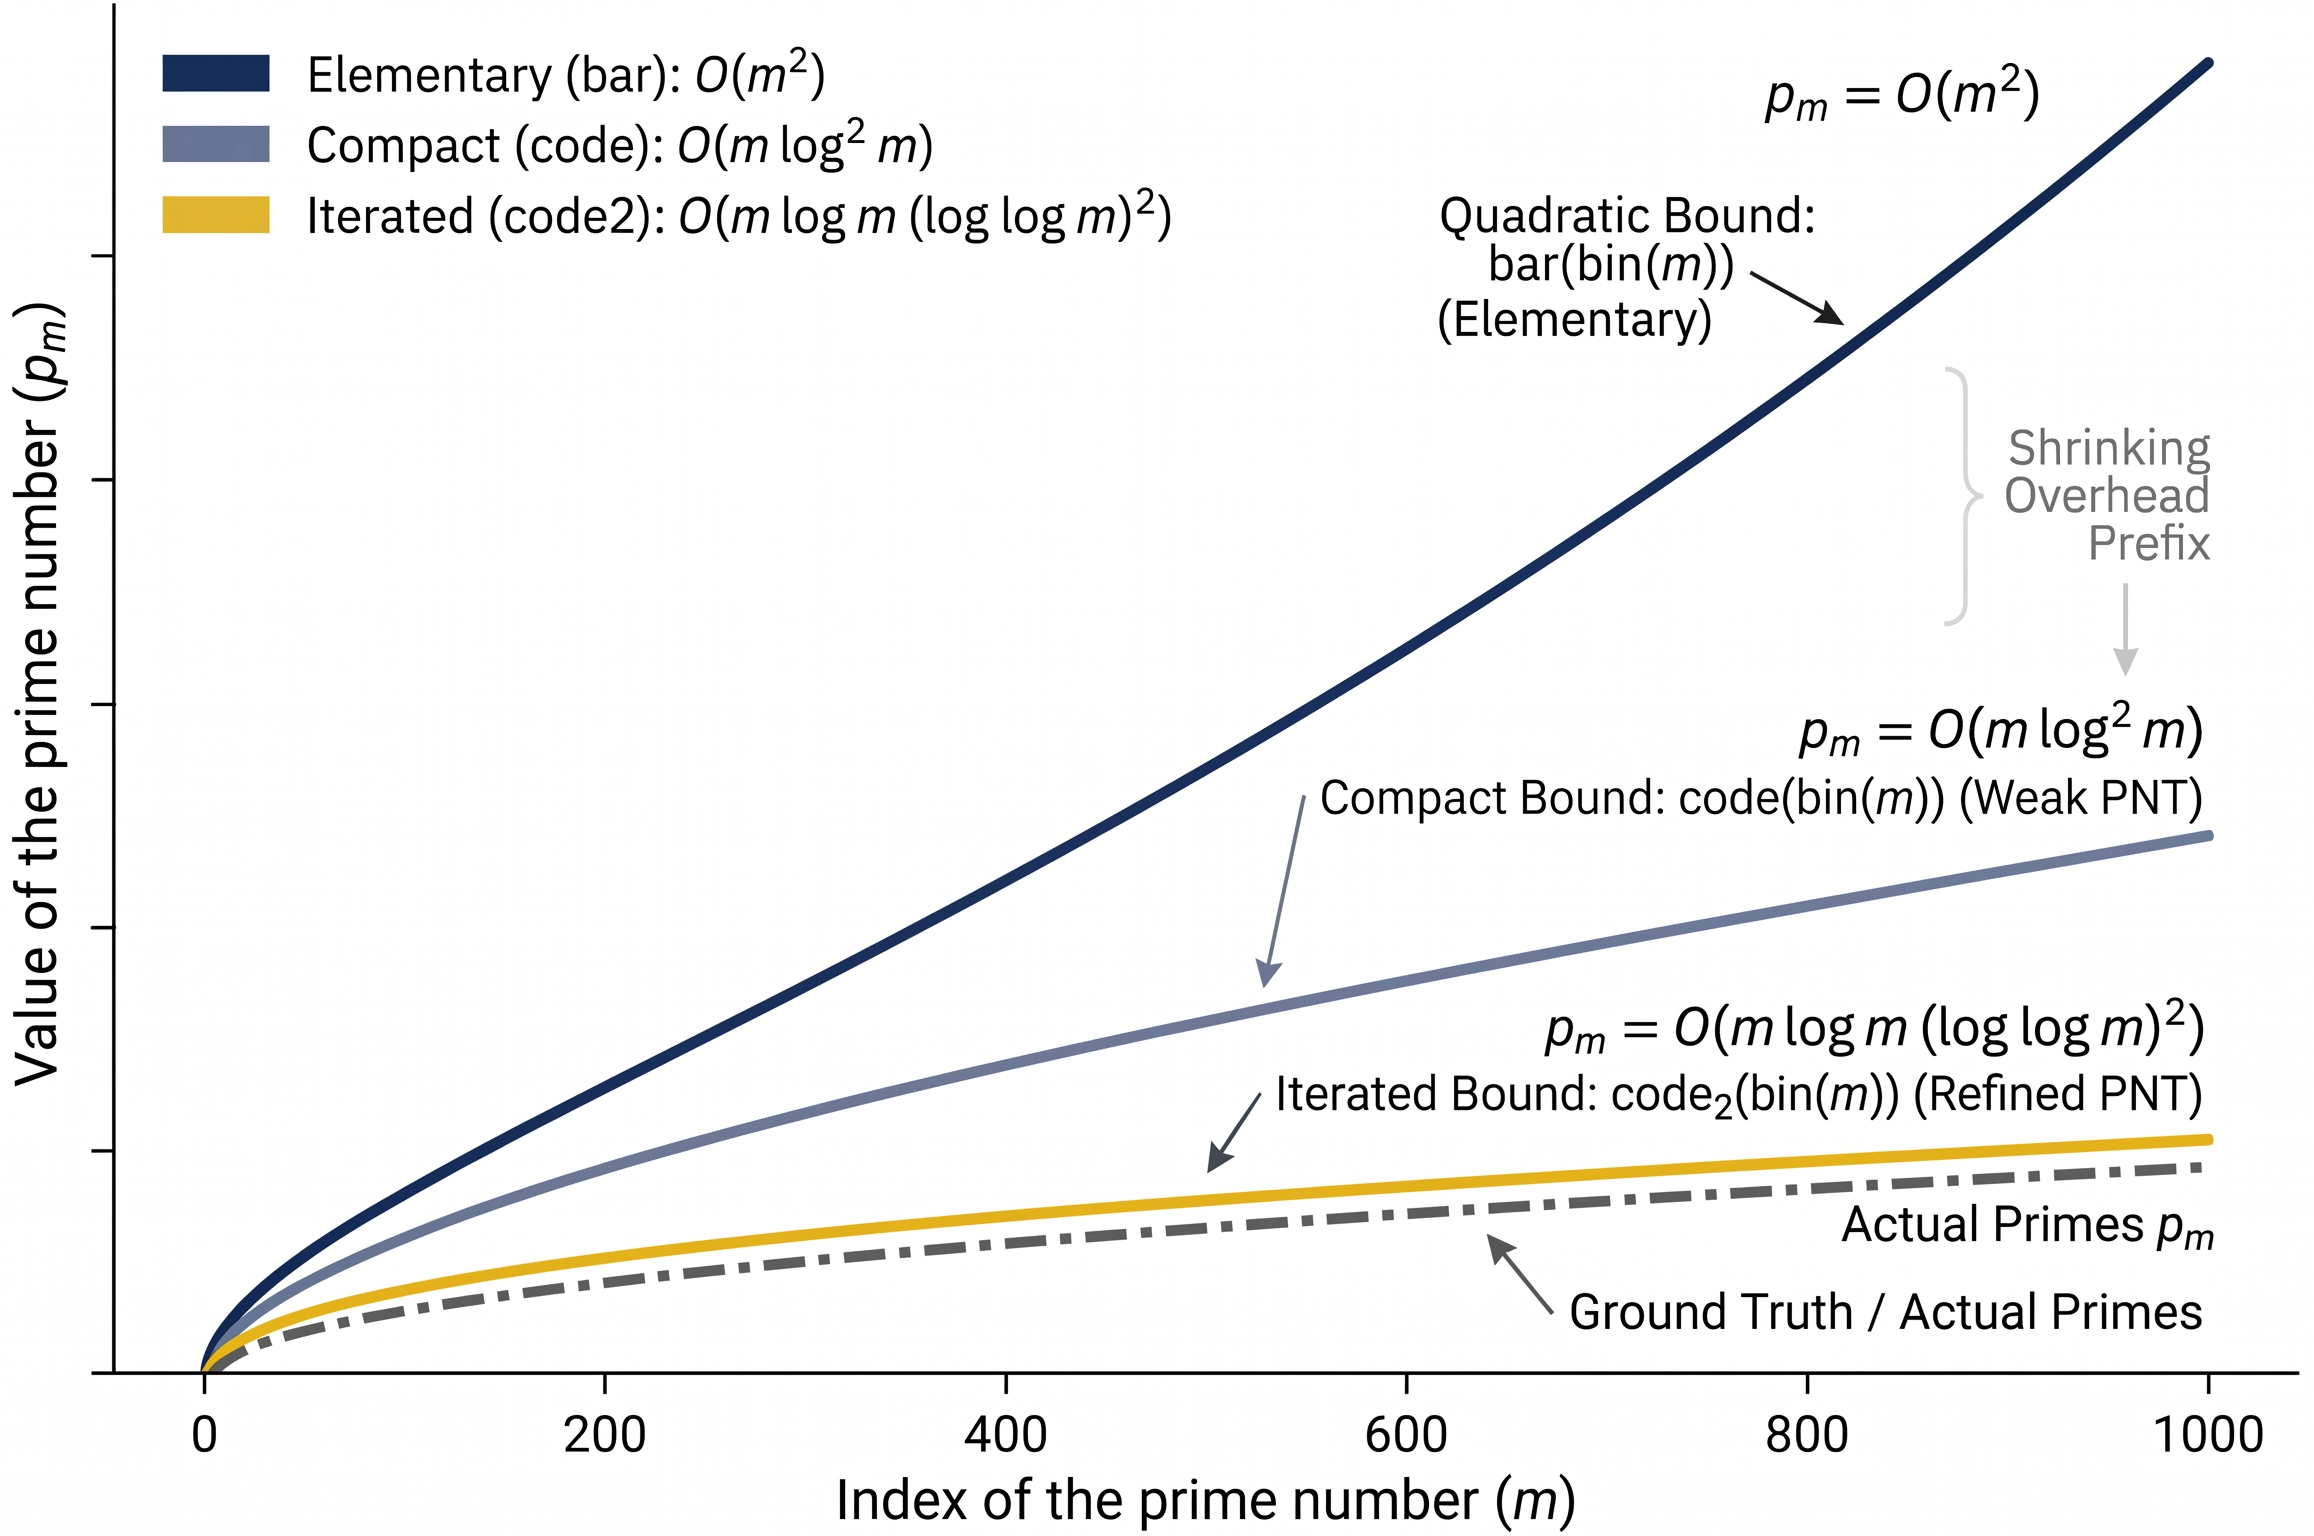
\includegraphics[height=0.68\textheight]{figures/asymptotic_bounds.jpeg}
        \caption{\footnotesize{Cotas superiores para $p_m$ derivadas dos três códigos: $\mathcal{O}(m^2)$ (elementar), $\mathcal{O}(m \log_2^2 m)$ (compacto, Weak PNT) e $\mathcal{O}(m \log_2 m (\log_2\log_2 m)^2)$ (iterado), cada vez mais próximas dos primos reais.}}
        \label{fig:asymptotic_bounds}
    \end{figure}
\end{frame}

\begin{frame}{Não-Vacuidade e a Interface Church--Turing}
    \begin{enumerate}
        \item \textbf{Existência de palavras incompressíveis (\texttt{h\_incomp}):} \texttt{exists\_incompressible\_word} usa o argumento de contagem da \texttt{Complexitylib} para provar que, para todo método $M$ e todo $\ell$, existe $w$ com $|w| = \ell$ e $|w| \le M.\text{ecomplexity}(w)$;
        \medskip
        \item \textbf{Sobrecarga de descrição (\texttt{h\_desc}):} na \texttt{Complexitylib}, um \texttt{DescriptionMethod} é uma função parcial arbitrária, e não uma máquina concreta. A formalização prova mecanicamente:
        \begin{itemize}
            \item \texttt{encodePairCode\_inj}: o par $(m, k)$ é recuperável da fita;
            \item \texttt{reconstructFromPrime\_div}: $p_m \cdot (n/p_m) = n$.
        \end{itemize}
        Pelo Teorema da Invariância \cite{li2019introduction}, o descompressor correspondente custa apenas uma constante de $c$ bits.
    \end{enumerate}
    \begin{tcolorbox}[pucbox, title=Separação de Responsabilidades]
        \small O postulado de computabilidade fica explícito na assinatura (constante $c$), enquanto \textbf{100\%} das deduções aritméticas, logarítmicas e de códigos são verificadas pelo \textit{kernel} do Lean 4.
    \end{tcolorbox}
\end{frame}

\begin{frame}{Entregáveis}
    Dentro do escopo das atividades propostas em \citeonline{schoning1998kolmogorov}, foram concluídos os seguintes entregáveis:
    \medskip

    \begin{tcolorbox}[pucbox, title=Entregáveis do Projeto]
        \begin{itemize}
            \item[$\checkmark$] Cinco módulos Lean 4 com definições, lemas e teoremas dos Exercícios 9.1--9.5, \textbf{formalmente verificados e livres de \texttt{sorry}};
            \item[$\checkmark$] Código organizado, documentado e reproduzível (\texttt{lake build}) em um repositório público no GitHub;
            \item[$\checkmark$] Relatório técnico (formato ACM) com o detalhamento passo a passo da formalização.
        \end{itemize}
    \end{tcolorbox}
\end{frame}

\section[Considerações Finais]{Considerações Finais}

\begin{frame}{Considerações Finais}
    \begin{itemize}
        \item O objetivo principal foi \textbf{integralmente alcançado}: o Teorema Fraco dos Primos e seu refinamento iterado foram provados em Lean 4, passo a passo e \textbf{sem nenhum \texttt{sorry}};
        \medskip
        \item O fator ``fraco'' $\log_2 n$ foi \textbf{explicado formalmente}: é o custo do cabeçalho livre de prefixo, e cada nível de compressão do cabeçalho aperta a cota;
        \medskip
        \item A ponte \texttt{Mathlib} $\leftrightarrow$ \texttt{Complexitylib} (\texttt{BinWord}, códigos autodelimitados e reconstrução aritmética) é \textbf{reutilizável} em outros argumentos de incompressibilidade;
        \medskip
        \item Passos implícitos nos livros (concatenação sem perdas, aritmética de $\lfloor\log_2\rfloor$) tornaram-se \textbf{garantias verificadas por máquina}.
    \end{itemize}
\end{frame}

\begin{frame}{Trabalhos Futuros}
    \begin{enumerate}
        \item \textbf{Código $\omega$ de Elias e a $k$-ésima cota iterada:} formalizar o código recursivo de \citeonline{elias1975universal} para obter, num único teorema,
        \begin{equation*}
            p_m = \mathcal{O}\big(m \log_2 m \, \log_2^{(2)} m \cdots (\log_2^{(k)} m)^2\big);
        \end{equation*}
        \item \textbf{Teorema da Invariância concreto no CSLib:} construir um interpretador concreto (máquina de registradores ou $\lambda$-cálculo), provar a invariância e eliminar a hipótese \texttt{h\_desc};
        \medskip
        \item \textbf{Framework geral de incompressibilidade:} abstrair o pareamento livre de prefixo e os lemas de contagem num módulo/tática reutilizável, para formalizar cotas em números de Ramsey, torneios, lemas de bombeamento e complexidade de circuitos \cite{li2019introduction}.
    \end{enumerate}
\end{frame}

% =========================================================================
\section{Referências}
% =========================================================================
\begin{frame}[allowframebreaks]{Referências}
    \bibliography{refs}
\end{frame}
\end{document}
